\documentclass[12pt,a4paper,ngerman]{report}
\usepackage{babel}
%\usepackage{natbib}
\usepackage{url}
%\usepackage[left=2cm, right=1.5cm, top=2cm, bottom=2cm]{geometry}
%\usepackage[ansinew]{inputenc}
\usepackage{amsmath}
\usepackage{nicefrac} % macht schöne Brüche mit querstrich mit \nicefrac{1}{2}
\usepackage{graphicx}
%\graphicspath{}
\usepackage{titlesec}% um chapterüberschriften anzupassen.
\titleformat{\chapter}{\normalfont\huge\bf}{\thechapter.}{20pt}{\huge\bf}
\usepackage{parskip}
\usepackage{fancyhdr}
\usepackage{amsfonts}
\usepackage{float}
\usepackage{caption}
\usepackage{subcaption} % for \begin{subfigure}
	
\usepackage{csquotes} % mit \enquote{blabla} tolle anfürungsstriche erstellen
%\usepackage{physics} %lässt mich \bra und \ket benuzen %im konflict mit siunitx

\usepackage{pgfplots} %für plots
\pgfplotsset{compat=newest}

\usepackage{varioref} % macht mit \vref{} viel bessere referenzen
\usepackage{hyperref} % macht klickbare referenzen

\usepackage{xcolor, soul} %mit \hl{} kann man toll Sachen hervorheben.
\newcommand{\highlight}[1]{%
	\colorbox{yellow!50}{$\displaystyle#1$}} % mit \highlight{} kann man sogar in Gleichungen hervorheben

\usepackage{vmargin}
\usepackage[section]{placeins}
\usepackage{capt-of}
\usepackage{enumitem}
\usepackage{multirow}
\usepackage{blindtext}
\usepackage[version=4]{mhchem} % um Chemische Elementsymbole zu benutzen: \ce{H20}

\usepackage{pdfpages} % um PDFs einzufügen

%spread to latex:
\usepackage{booktabs, multirow} % for borders and merged ranges
\usepackage{changepage,threeparttable} % for wide tables

\providecommand{\e}[1]{\ensuremath{\cdot 10^{#1}}}
\providecommand{\fehlt}{\textcolor{red}{\emph{Fehlt!\dots}}}

\usepackage{siunitx}
\sisetup{
	separate-uncertainty = true,
	%per-mode = fraction,
	%per-mode = symbol
	%locale = DE
}
\DeclareSIUnit\bar{bar}
\DeclareSIUnit\atomicmassunit{u}



\setmarginsrb{3 cm}{2.5 cm}{3 cm}{2.5 cm}{1 cm}{1.5 cm}{1 cm}{1.5 cm}
\title{UI-Kennlinien}		%%%%%%%%%% T I T L E %%%%%%%%%%
% Title / Titel


\author{Frederik Uhlemann, F. Adamczyk}
% Author
\date{\today}
% Date

\makeatletter
\let\thetitle\@title
\let\theauthor\@author
\let\thedate\@date
\makeatother

\pagestyle{fancy}
\fancyhf{}
\rhead{\theauthor}
\lhead{UI-Kennlinien}
\cfoot{\thepage}
%%%%%%%%%%%%%%%%%%%%%%%%%%%%%%%%%%%%%%%%%%%%
\begin{document}
		
	%%%%%%%%%%%%%%%%%%%%%%%%%%%%%%%%%%%%%%%%%%%%%%%%%%%%%%%%%%%%%%%%%%%%%%%%%%%%%%%%%%%%%%%%%
	
	\begin{titlepage}
		\centering
		\vspace*{0.5 cm}
		% \begin{large} Justus-Liebig-Universität\\ Gießen \end{large}
		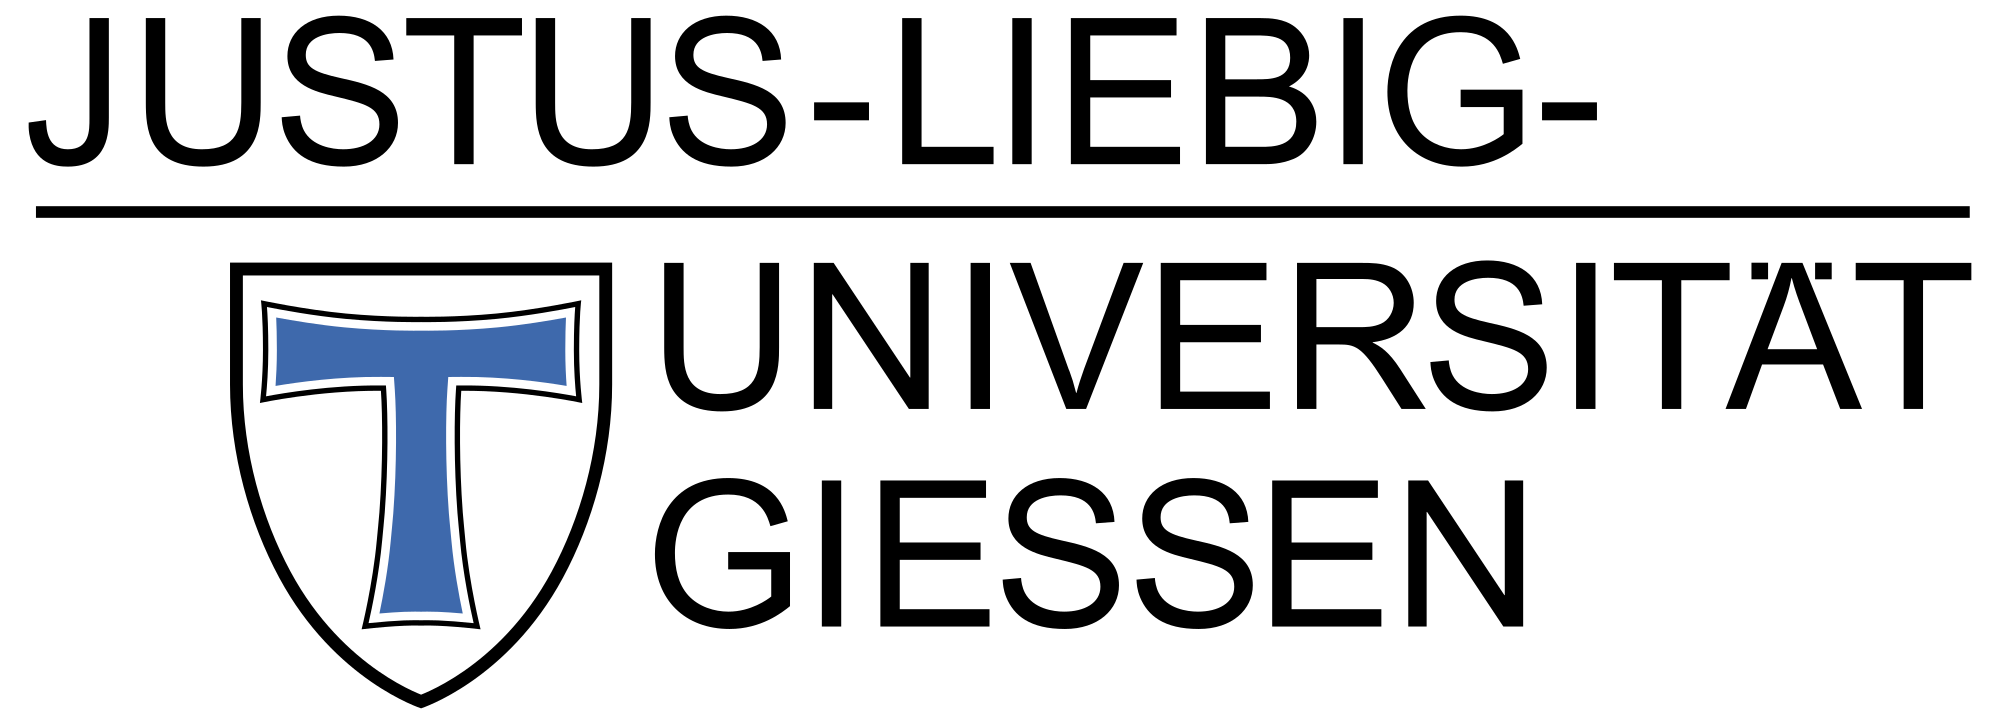
\includegraphics[width = 0.6 \textwidth]{JLU_Giessen-Logo}	%University Logo
		\\[2.0 cm]
		% \begin{center}    \textsc{\Large Justus - Liebig - Universität}\\{Giessen}\\[0.8cm]	\end{center}% University Name
		Versuch 4 des\\
		\textsc{\Large  Fortgeschrittenen-Praktikums}\\ [0.3 cm]				% Course Code
		\rule{\linewidth}{0.2 mm} \\[0.4 cm]
		{ \huge \bfseries \thetitle}\\%%% TITEL HERE
		\rule{\linewidth}{0.2 mm}\\
		Versuchstermin Freitag, 17.05.2024 \\
		~\\
		[2.0 cm]
		
		
		\begin{minipage}{0.49\textwidth}
			\begin{flushleft}
				\emph{Praktikumsbetreuer:}\\
				Marius Müller\\
				%  Affiliation\\
				\small{\href{mailto:marius.mueller@physik.uni-giessen.de}{marius.mueller@physik.uni-giessen.de}}
			\end{flushleft}
		\end{minipage}~
		\begin{minipage}{0.49\textwidth}
			\begin{flushright}
				\emph{Protokoll von:} \\
				
				\large{Frederik Uhlemann}\\
				\small{\href{mailto:frederik-vincent.uhlemann@physik.uni-giessen.de}{frederik-vincent.uhlemann@physik.uni-giessen.de}\\~\\
					%Matrikel Nr.: \:  \\[0.5cm]
					%\href{mailto:}{}
				}
				\large{Florian Adamczyk} \\
				\small{\href{mailto:florian.marius.adamczyk@physik.uni-giessen.de}{florian.marius.adamczyk@physik.uni-giessen.de}\\
					%Matrikel Nr.: \: 8105234}
			}
		\end{flushright}
	\end{minipage}
	
	\end{titlepage}
	
%%%%%%%%%%%%%%%%%%%%%%%%%%%%%%%%%%%%%%%%%%%%%%%%%%%%%%%%%%%%%%%%%%%%%%%%%%%%%%%%%%%%%%%%%
\setcounter{secnumdepth}{3}
\setcounter{tocdepth}{4}
\tableofcontents
%\newpage

%%%%%%%%%%%%%%%%%%%%%%%%%%%%%%%%%%%%%%%%%%%%%%%%%%%%%%%%%%%%%%%%%%%%%%%%%%%%%%%%%%%%%%%%%
%\renewcommand{\thesection}{\arabic{section}} %lässt in den subsections die erste zahl von darüberliegenden chapter weg.

%\pagebreak
	
%\setcounter{chapter}{-1}
\chapter*{Einleitung}
	\addcontentsline{toc}{chapter}{Einleitung}
	
	In der Welt der Elektronik sind die Charakteristiken von Halbleiterbauteilen von entscheidender Bedeutung. Dieser Versuch zielt darauf ab, die typischen Kennlinien einer Diode, eines Bipolartransistors und eines Feldeffekttransistors zu erfassen, um ihre spezifischen Eigenschaften und Verhaltensweisen zu verstehen. Zusätzlich liegt ein Fokus auf der Untersuchung von Solarzellen, bei denen durch die Aufnahme von Dunkel- und Hell-Kennlinien wichtige Kenngrößen ermittelt werden sollen. Die Ergebnisse sollen nicht nur Aufschluss über den Typ der Dioden und Transistoren geben, sondern auch über die Leistungsfähigkeit der Solarzellen, wie etwa den Füllfaktor und die relative Effizienz.



\chapter{Versuchsaufbau und Durchführung}
	In den Versuchen werden die Kennlinien der Halbleiterbauteile aufgenommen. Dazu werden die fertigen Schaltungen mit dem Messgerät farblich passend verbunden und die Kennlinien mit einem LABVIEW-Programm aufgenommen und auf einen USB-Stick abgespeichert. So können die Daten später ausgewertet werden.\\

	\begin{itemize}
	\item[-] Im ersten Versuchsteil wird die Kennlinie einer Diode aufgenommen. Dazu wird die Diode in Durchlassrichtung und in Sperrrichtung betrieben.
	\item[-] Im zweiten Versuchsteil wird die Kennlinie eines Bipolartransistors aufgenommen. Dazu wird der Transistor in der Emitterschaltung betrieben und die vier Kennlinienfelder aufgenommen.
	\item[-] Im dritten Versuchsteil wird die Kennlinie eines Feldeffekttransistors aufgenommen. Dazu wird der Transistor in der Source-Schaltung betrieben und die vier Kennlinienfelder aufgenommen.
	\item[-] Im vierten Versuchsteil werden zwei Solarzellen untersucht. Dazu wird die Kennlinie der Solarzellen im Dunkeln und im Licht aufgenommen und die jeweiligen Kennlinien abgespeichert.
	\end{itemize}

\chapter{Auswertung}
	\section{Diode}
		Die Diodengleichung (oder auch Shockley-Gleichung) ist gegeben durch: 
		\begin{eqnarray}
		\label{eq:shockley}
		I_\text{D} = I_\text{S}(T) \, \left(\mathrm e^\frac{U}{n\,U_\text{T}} - 1 \right)
		\end{eqnarray}
		
		Dabei bezeichnet $I_\text{S}(T)$ den Sättigungssperrstrom welcher typischerweise zwischen \qty{10e-12}{\ampere} und \qty{10e-6}{\ampere} liegt, $ U_\text{T}= \frac{k \cdot T} q$ die Tem\-pe\-ra\-tur\-span\-nung und $n$ den Idealitätsfaktor oder Emissionskoeffizient. Dieser soll auch bestimmt werden und liegt typischerweise zwischen 1 und 2.\\ 
		In unserem Fall (bei Raumtemperatur von \qty{25}{\celsius}) beträgt die Temperaturspannung  $U_T = \qty{25}{\milli\volt}$.
		
		\begin{figure}
			\centering
			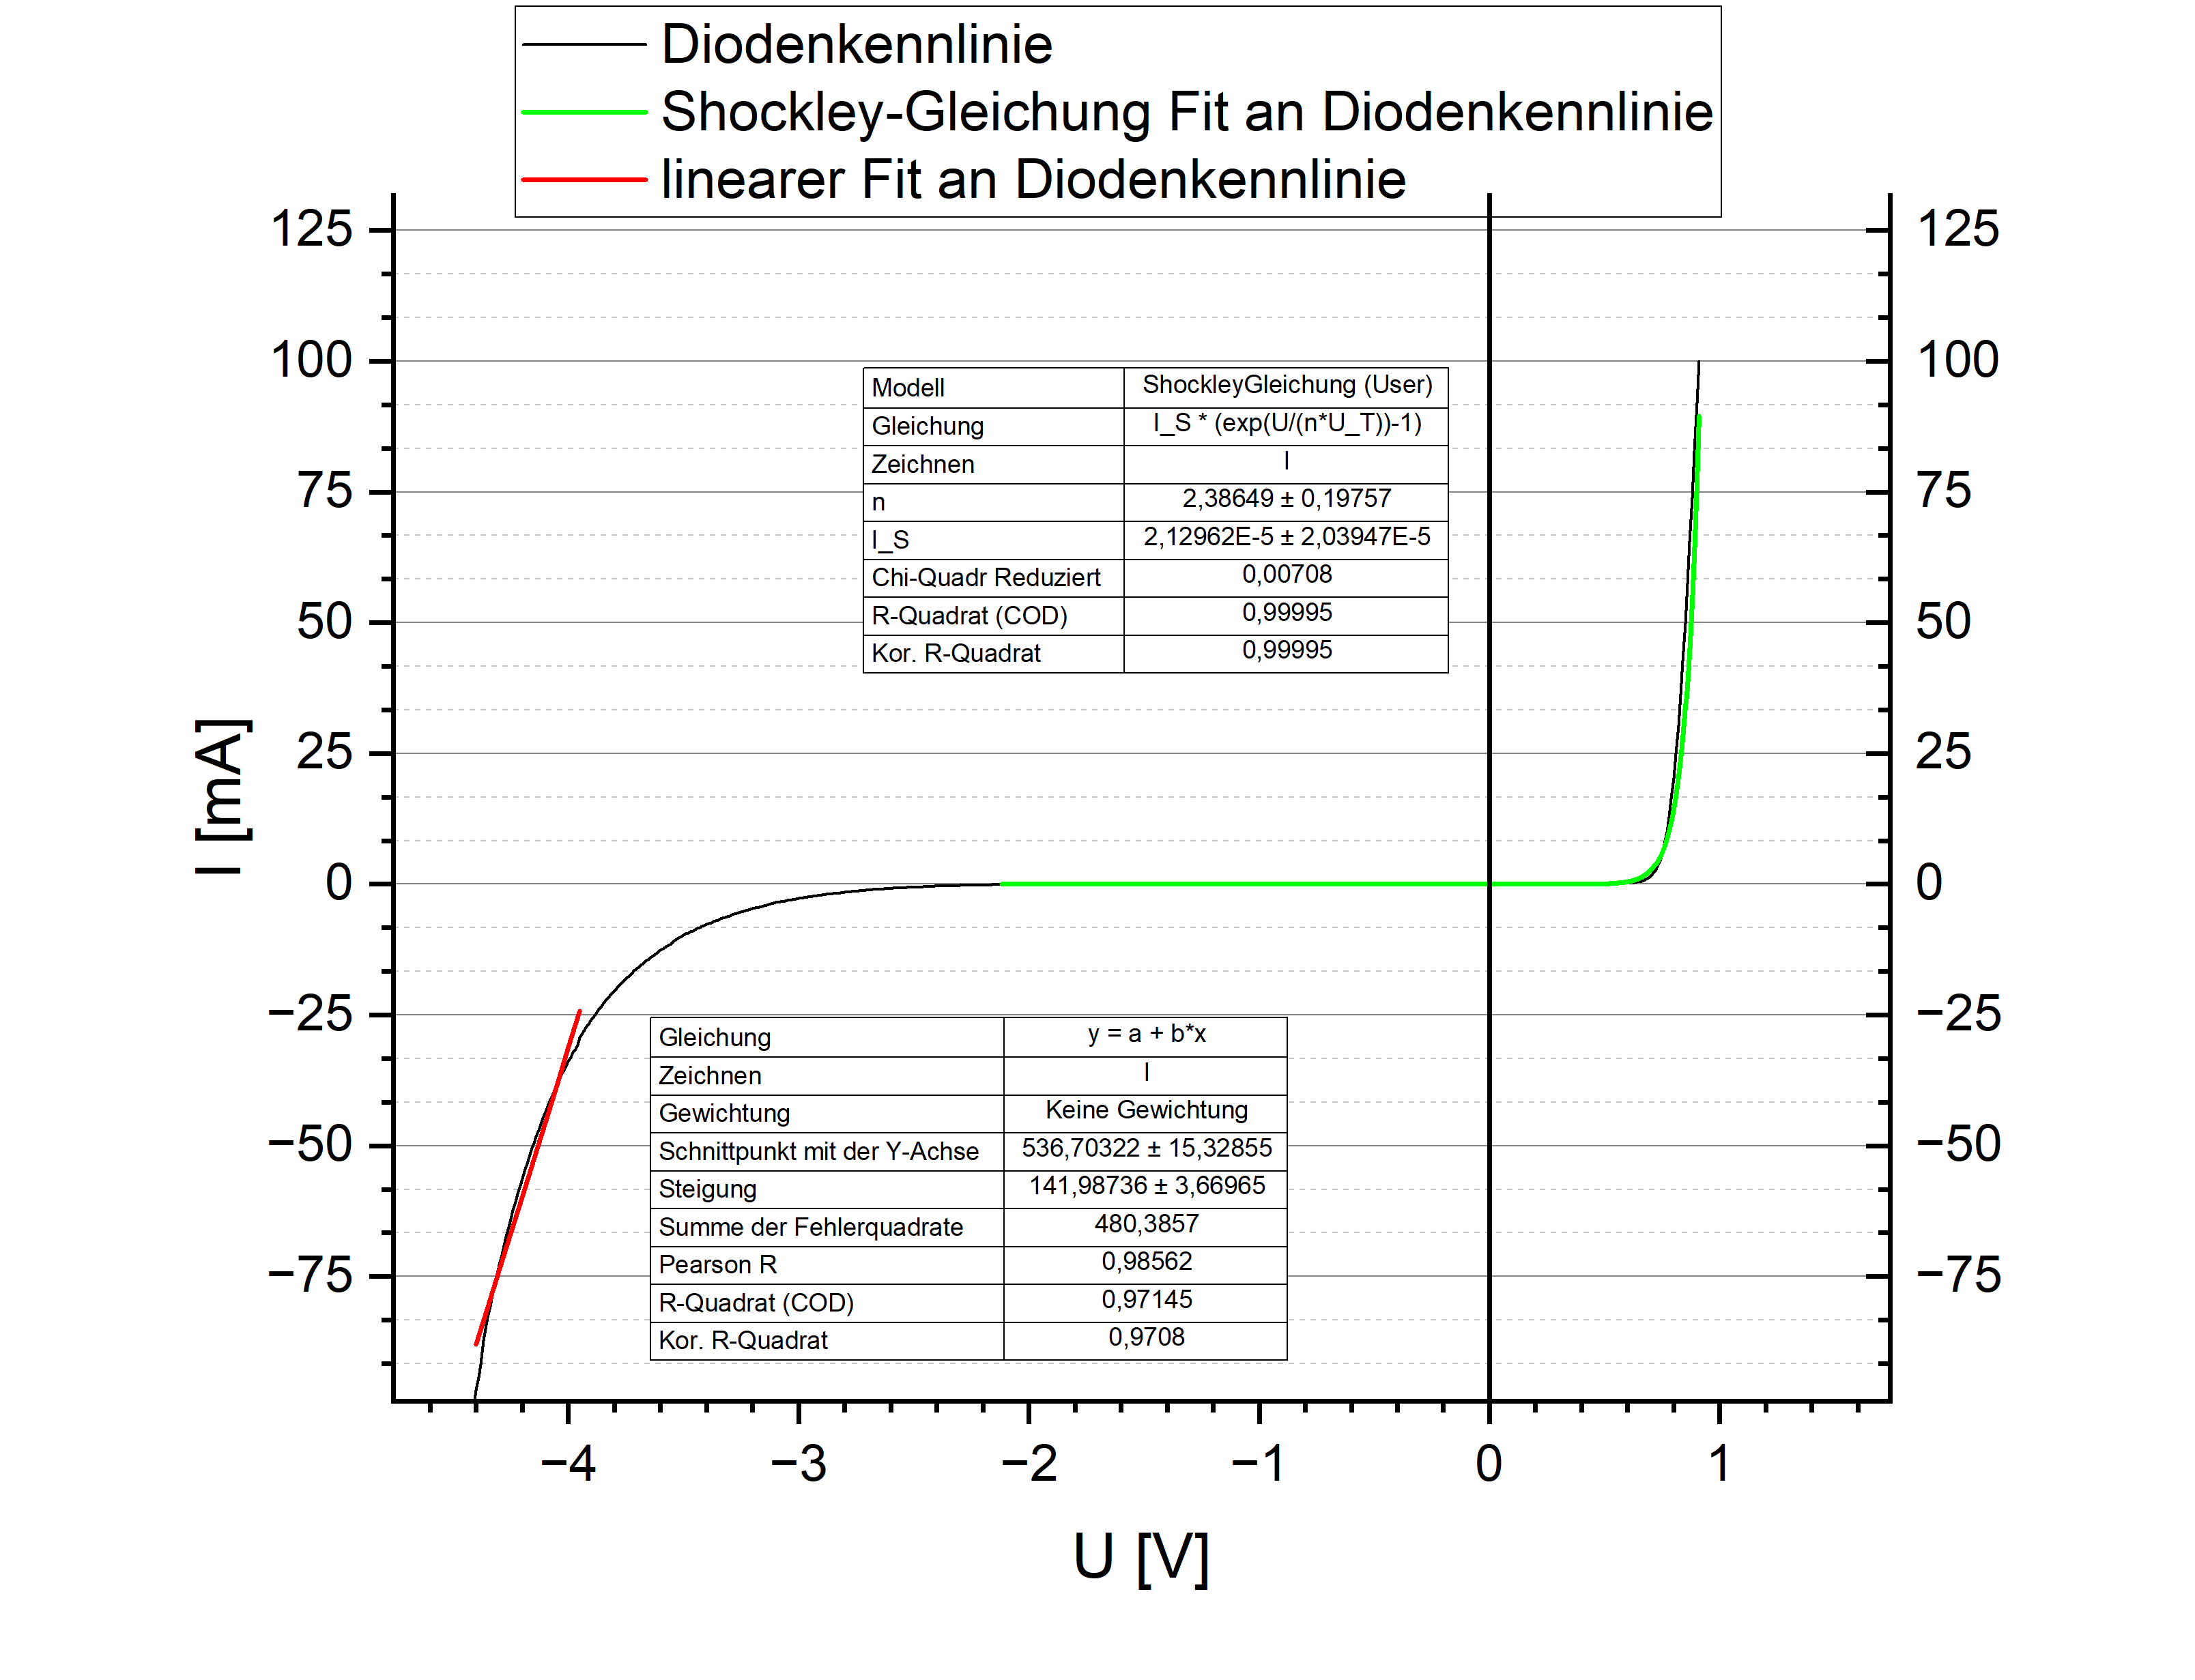
\includegraphics[width=0.8\textwidth]{Origin/Graph1.png}
			\caption{Kennlinie der Diode}
			\label{fig:Diodenkennlinie}
		\end{figure}

		In Abbildung \ref{fig:Diodenkennlinie} ist die Kennlinie der Diode dargestellt. \\ 
		Der rechte Teil der Kennlinie ist mit der Gleichung \ref{eq:shockley} gefittet worden, während der linke Teil nicht mit dieser Gleichung beschrieben werden kann und daher linear gefittet ist. \\

		Im Schockley-Fit kann man den Sättigungssperrstrom $I_\text{S}$ und den Idealitätsfaktor $n$ bestimmen. Daraus ergibt sich:
		\begin{itemize}
			\item Sättigungssperrstrom $I_\text{S} = \SI{2.129 +- 2.0394 e-2}{\micro\ampere}$
			\item Emissionskoeffizient $n = \num{2.386 +- 0.198} $
		\end{itemize}

		Um die Durchbruchspannung zu bestimmen, betrachten wir den linearen Fit auf der rechten Seite des Diagramms. Davon müssen wir den Schnittpunkt mit der x-Achse (bzw. Spannungsachse) bestimmen.
		Dazu setzen wir die Gleichung\\
		$I=B \cdot U_D + A \stackrel{!}{=} 0$. Hieraus ergibt sich dann:
		$$U_D = \frac{-a}{b}  = \frac{-536.703}{141.987} = \qty{3.77}{\volt}$$

		Aus Origin werden folgende Fehler für $b$ und $a$ gegeben:\\ $\Delta b = \pm 3,670 $ und $\Delta a = \pm 15,329$.

		Durch Fehlerfortpflanzung erlangen wir:
		\begin{eqnarray}
			\Delta U =\left|\frac{\partial U_D}{\partial b}\right| \Delta b + \left|\frac{\partial U_D}{\partial a}\right|\Delta a = \left|\frac{a\Delta b}{b^2}\right|  + \left|\frac{\Delta a}{b}\right| \approx 0,21 \mathrm{V}
		\end{eqnarray}


		Die bestimmte Durchschlagsspannung ist also:
			\[ U_D = \qty{3.77 +- 0.21}{\volt}\]

		Dieser Wert lässt darauf schließen, dass es sich bei der untersuchten Diode um eine Zener-Diode handelt: Diese Dioden werden beim Betrieb in Sperrrichtung nicht zerstört und
		lassen sich beispielsweise als Spannungsstabilisatoren einsetzen.

		
	\section{Bipolartransistor}
		\begin{figure}[ht]
			\centering
			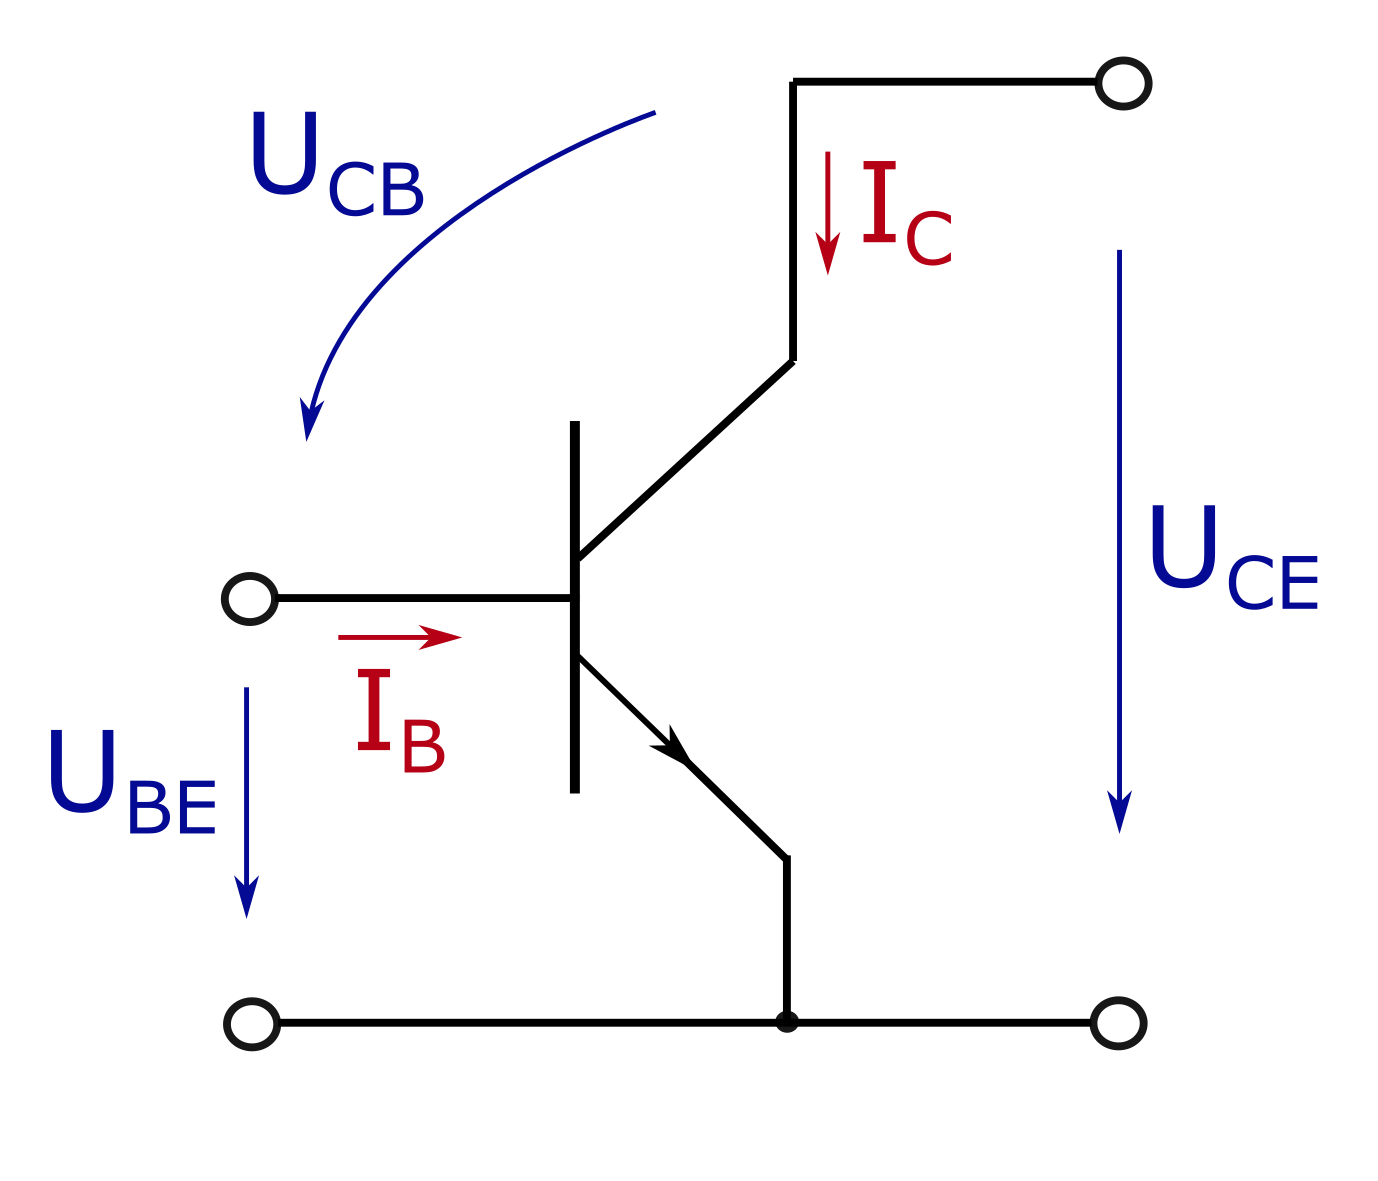
\includegraphics[width=7.5 cm]{plots/transistor_schaltung.png}
			\caption{Schaltskizze eines pnp-Transistors}
			\label{img:pnpSchaltung}
		\end{figure} 
		Im folgenden Versuchsteil werden die typischen Kennlinienfelder eines Bipolartransistors vermessen. Es handelt sich um einen pnp-Transistor des Typs BC550. Ein Schaltplan solch eines Transistors ist in Abbildung \ref{img:pnpSchaltung} dargestellt. Dabei sind die wichtigsten Größen eingetragen, dazu zählen der Kollektor- und Basisstrom $I_C$ und $I_B$, zudem die jeweiligen Spannungen zwischen Kollektor, Emitter und Basis. 
		\subsection{Vierpolarparameter}
				\begin{figure}[h]
			\centering
			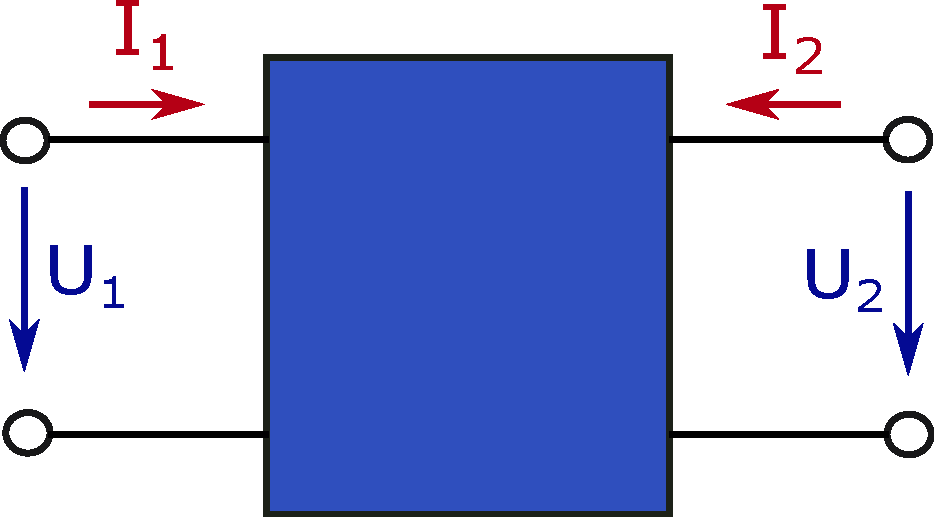
\includegraphics[width=7.5 cm]{plots/Vierpol.pdf}
			\caption{allgemeiner Vierpol}
			\label{img:Vierpol}
		\end{figure} 
		Jedes elektronische Bauteil kann als Vierpol dargestellt werden, in Abbildung \ref{img:Vierpol} ist der Schaltplan eines allgemeinen Vierpols angegeben. Das Modell beschreibt ein elektrisches Netzwerk oder Bauteil durch zwei Ein- und Ausgänge, dabei wird ein lineares Gleichungssystem mit einer 2x2 Matrix verwendet.\\
		Transistoren sind aktive Bauelemente und nicht linear, deshalb müssen sie in einem Punkt linearisiert werden, damit die Beschreibung des Vierpols angewandt werden kann. Dieser Punkt heißt Arbeitspunkt des Transistors. Für Transistoren in der Emittersschaltung wird häufig die folgende Hybrid-Darstellung verwendet:
		\begin{equation}
			\begin{pmatrix}
				u_{BE}\\
				i_C
			\end{pmatrix}
		=	\begin{pmatrix}
				h_{11} & h_{12}\\
				h_{21} & h_{22}\\
			\end{pmatrix}
		=	\begin{pmatrix}
				i_{B}\\
				u_{CE}
			\end{pmatrix}
		\end{equation}
		Wie bereits erwähnt wird am Arbeitspunkt des Transistors linearisiert, deshalb sind die Vierpolparameter Ableitungen in der folgenden Form:
		\begin{equation}
			\begin{split}
				h_{11} = \frac{\partial U_{BE}}{\partial I_{B}} \qquad h_{12} = \frac{\partial U_{BE}}{\partial U_{CE}}\\
				h_{21} = \frac{\partial I_{C}}{\partial I_{B}} \qquad h_{22} = \frac{\partial I_{C}}{\partial U_{CE}}\\
			\end{split}
		\end{equation}
		\subsection{Bestimmung der Parameter}
	\begin{figure}[h]
			\centering
			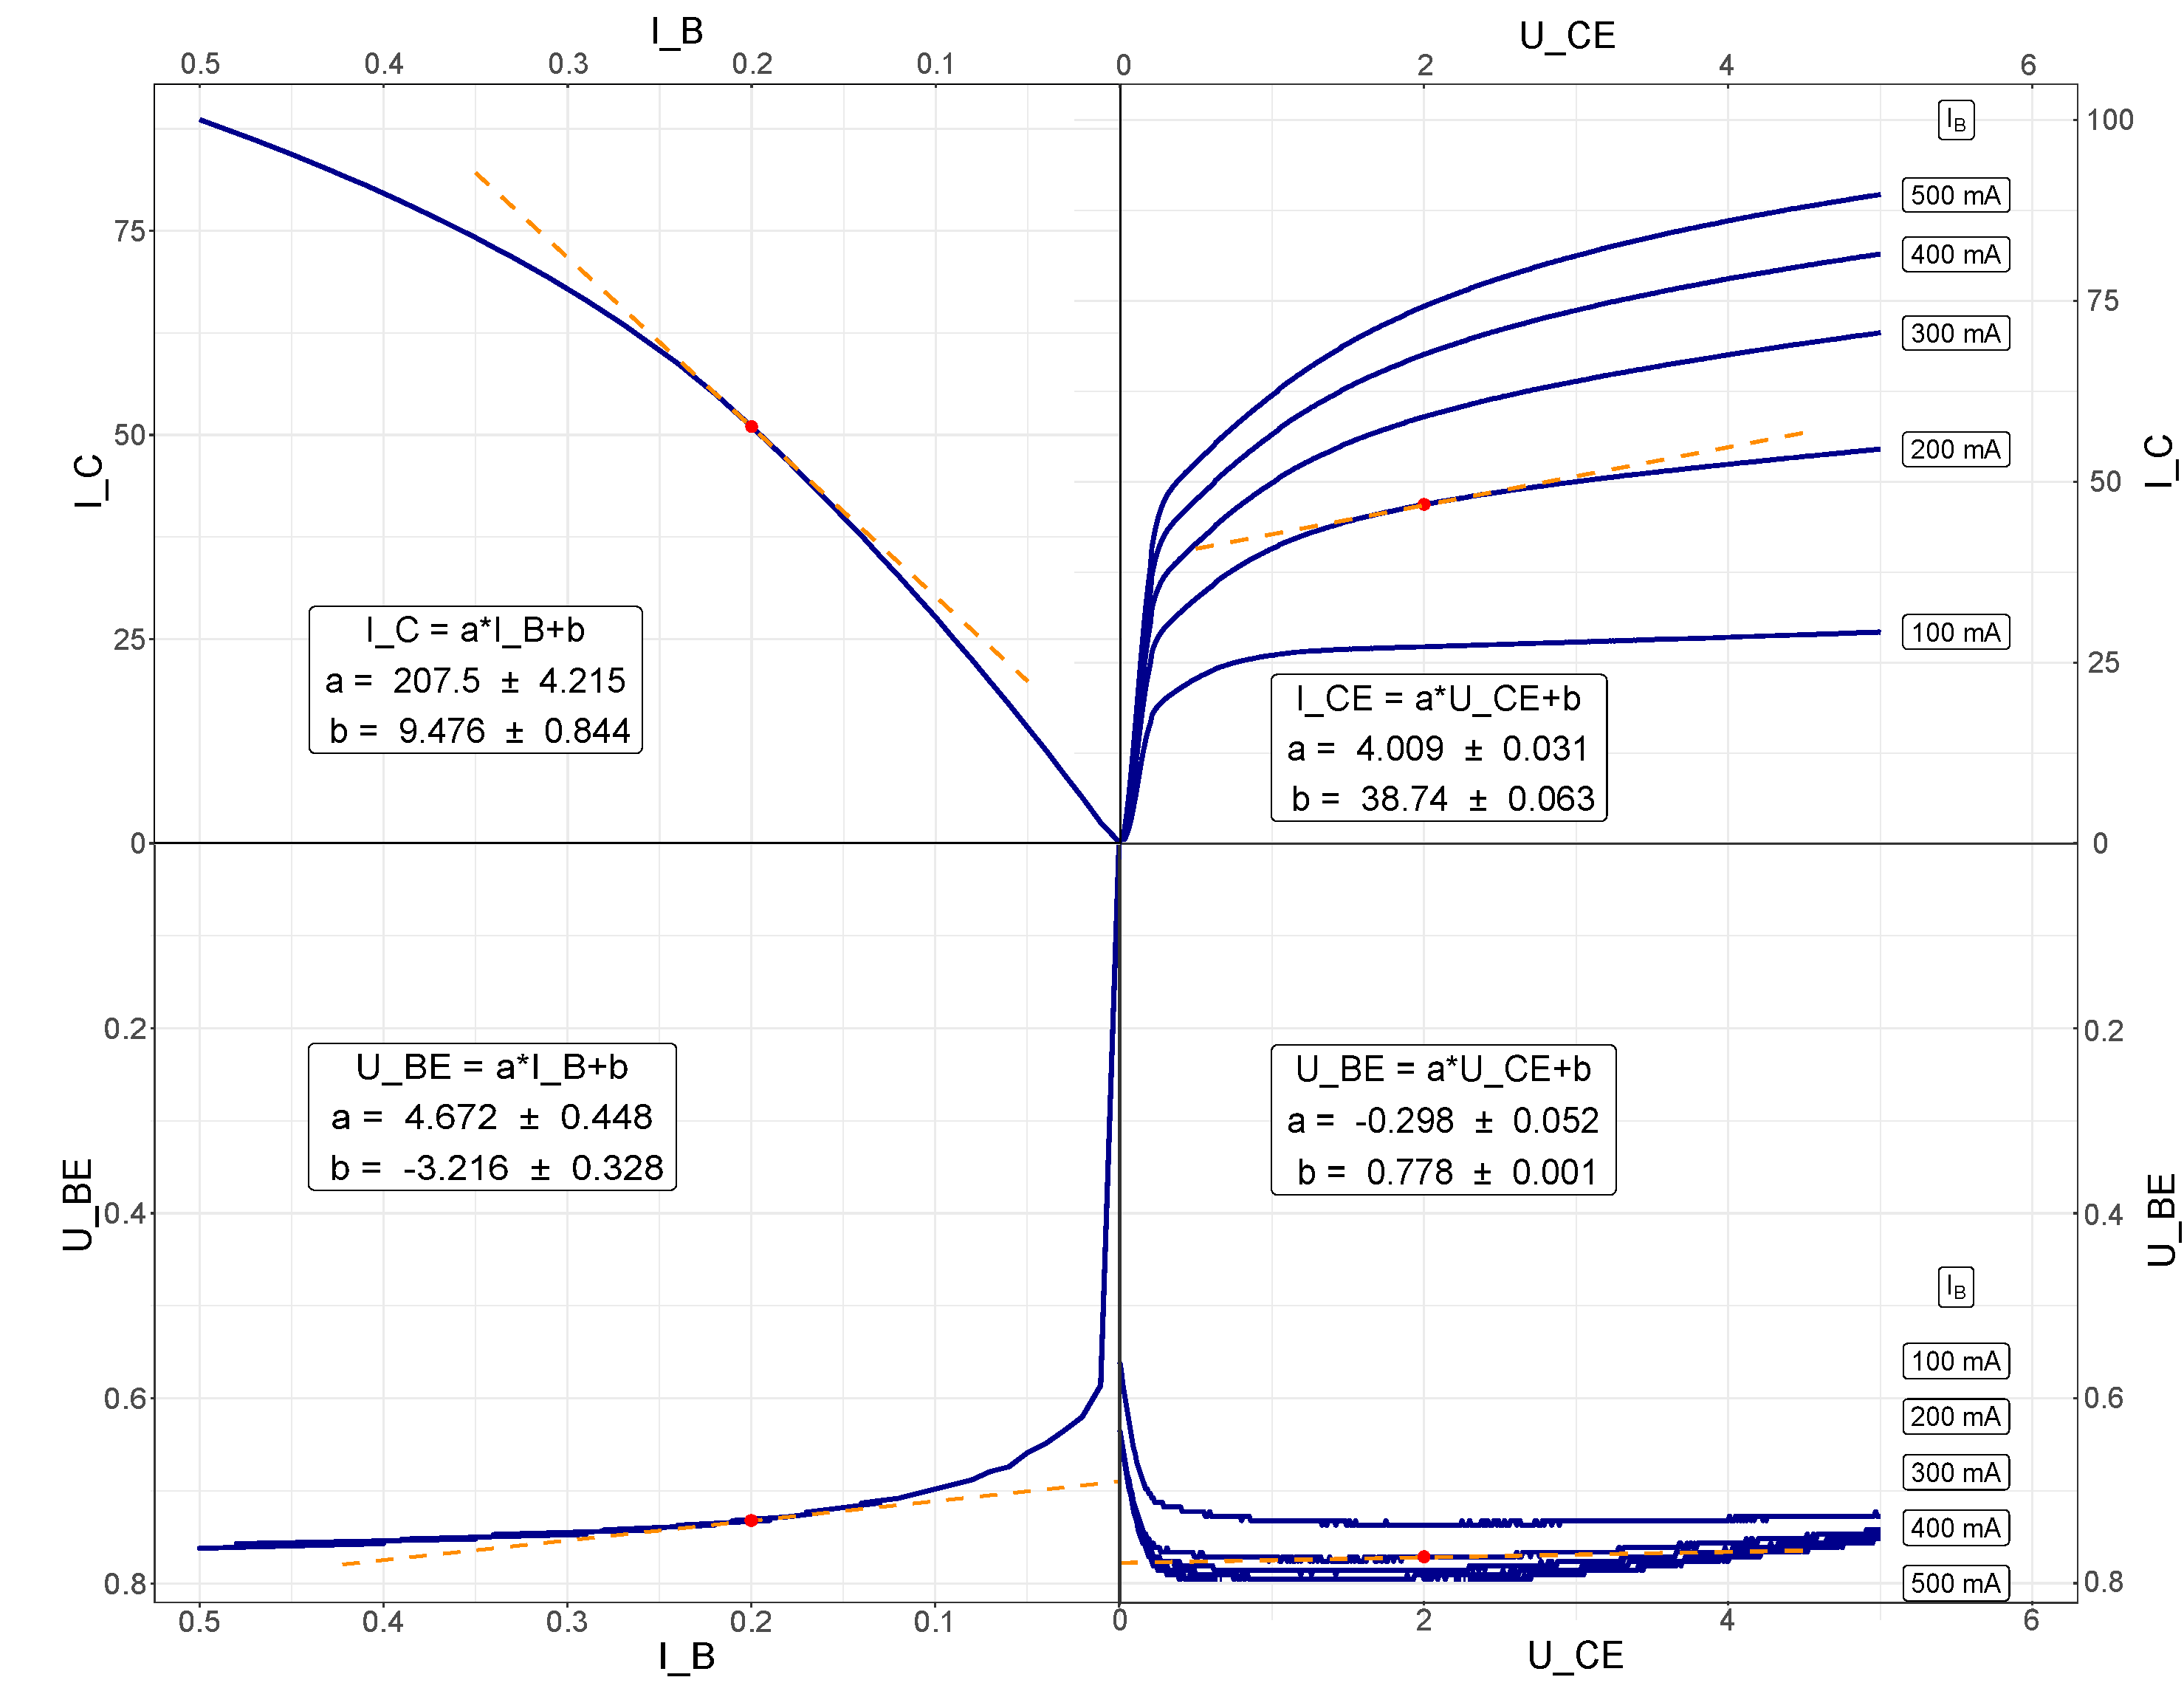
\includegraphics[width=\textwidth]{plots/Vierquadrantenkennlinienfeld.pdf}
			\caption{Vierquadrantenkennlinienfeld des Bipolartransistors}
			\label{img:Vierquadranten}
	\end{figure}
	In Abbildung \ref{img:Vierquadranten} sind die aufgenommenen, typischen vier Kennlinien des Transistors aufgetragen. In Rot ist jeweils der gewählte Arbeitspunkt eingetragen, dieser wird bei folgenden Werten gewählt:
	\begin{equation}
		I_B = \SI{0.2}{\milli \ampere} \qquad U_{CE} = \SI{2}{\volt}
	\end{equation}
	Zudem ist in Orange die jeweilige Fit-Gerade eingezeichnet und die Fitparameter sind gegeben.\\
	Der erste Vierpolparameter ergibt sich aus den Eingangskennlinien, also der $U_{BE}$-$I_B$ Kennlinie. Dieser Parameter ist direkt der differentielle Transistor-Eingangswiderstand:
	\begin{equation}
		r_{BE} = \frac{\Delta U_{BE}}{\Delta I_{B}}
	\end{equation}
	Im obigen Kennlinienfeld wurde die Gerade in einem Bereich von \SI{0.05}{\milli \ampere} um den Arbeitspunkt für $I_B$ zu $U_{BE}$ gefittet. Der differentielle Eingangswiderstand ist damit der Kehrwert des Fitparameters $a$, zudem werden die \si{\milli \ampere} in \si{\ampere} umgerechnet, um die Einheit \si{\ohm} zu erhalten:
	\begin{equation}
		r_{BE} = \frac{1}{a} = \underline{\SI{214.041(20.525)}{\ohm} = h_{11}}
	\end{equation}
	Der Vierpolparameter $h_{22}$ kann im Ausgangskennlinienfeld über den differentiellen Transistor-Ausgangswiderstand bestimmt werden. Der Widerstand ist die Steigung des Fits, erneut werden die \si{\milli \ampere} in \si{\ampere} umgerechnet:
	\begin{equation}
		r_{CE} =  \frac{\Delta U_{CE}}{\Delta I_{C}} = \SI{4009(31)}{\ohm}
	\end{equation}
	Der dazugehörige Vierpolparameter berechnet sich aus dem Kehrwert des Ausgangswiderstands:
	\begin{equation}
		\underline{h_{22} = \SI{2.494(19)E-4}{1 \per \ohm}}
	\end{equation}
	Aus dem Stromsteuerungskennlinienfeld $I_C$-$I_B$ kann der differentielle Stromverstärkungsfaktor $\beta$ bestimmt werden. Dieser ist entspricht dem Anstieg der gefitteten Geraden und gibt in gewisser Weise an, um welchen Faktor der Transistor den Kollektorstrom verstärkt. Dieser Faktor ist auch der Vierpolparameter $h_{21}$:
	\begin{equation}
		\beta =  \frac{\Delta I_{C}}{\Delta I_{B}} = \underline{207.5 \pm 4.2 = h_{21}}
	\end{equation}
	Der letzte Vierpolparameter ist im Rückwirkungskennlinienfeld der differentielle Rückwirkungsfaktor $D$. Dieser gibt an, wie stark Änderungen der Ausgangsspannung $U_{CE}$ auf die Eingangsspannung $U_BE$ zurückwirken. Solche sind unerwünscht und sollen möglichst klein sein. 
	\begin{equation}
		 D = \frac{\Delta U_{BE}}{\Delta U_{CE}} = \underline{-0.298 \pm 0.052 = h_{12}}
	\end{equation}

	\section{Feldeffektransistor}
	\begin{figure}[h]
		\centering
		\includegraphics[width=\textwidth]{plots/MosFET.pdf}
		\caption{Grundlegender Aufbau eines Metall-Oxid-Feldeffekttransistors}
		\label{img:MosFET}
	\end{figure}	
	Die Abbildung \ref{img:MosFET} zeigt den Grundlegenden Aufbau eines MOS-FET, die drei Anschlüsse heißen Source, Drain und Gate. Wenn zwischen Gate und Source eine Spannung angelegt wird, bildet sich eine leitende Brücke zwischen Source und Drain aus. Für die Steuerung von $U_{GS}$ ist fast kein Strom notwendig, daher ist die Steuerung eines MOS-FET's quasi leistungslos möglich.\\
	\begin{figure}[h]
	\centering
	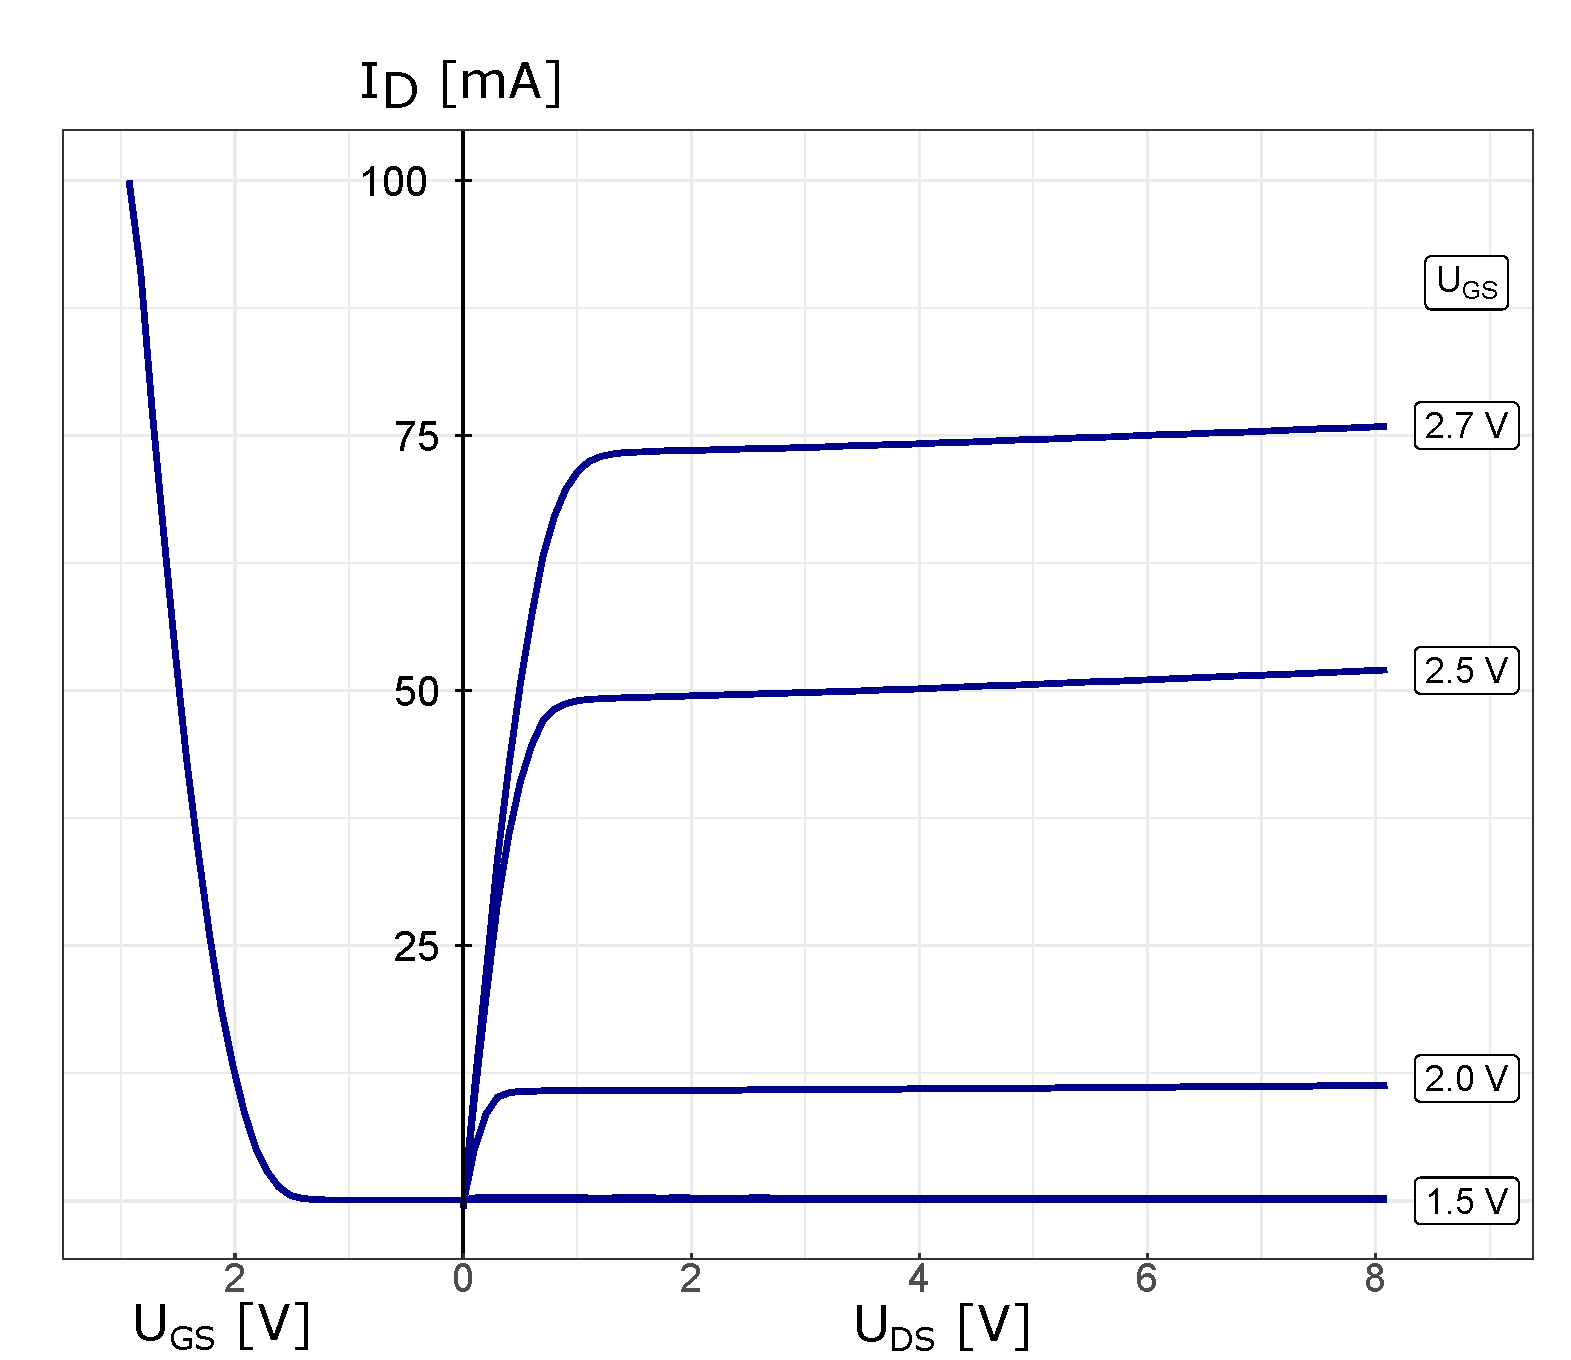
\includegraphics[width=\textwidth]{plots/FET.pdf}
	\caption{Kennlinienfelder des Feldeffektransistors}
	\label{img:FET}
	\end{figure}
	In Abbildung \ref{img:FET} sind die das $I_D$-$U_{DS}$ und $I_D$-$U_{GS}$ Kennlinienfeld, des Feldeffektransistors geplottet. Das erstere wird auch Ausgangskennlinienfeld genannt, es wurde für verschiedene Steuerspannungen $U_GS$ aufgezeichnet. Ab der Mindestgatespannung von etwas unter \SI{1}{\volt}, steigen die Kennlinien nur geringfügig an.\\
	Im linkem, dem Eingangkennlinienfeld wird deutlich, dass es sich tatsächlich um einen  Metall-Oxid-Feldeffekttransistors handelt, da der Strom $I_D$ bei einer Gate-Source-Spannung unter etwa \SI{1.4}{\volt} gleich null ist, der Transistor ist demnach selbstsperrend, danach steigt der Strom sprungartig an. Das $I_D$-$U_{GS}$ Kennlinienfeld zeigt die Steuerungseigenschaft des MOS-FET´s.
	\section{Solarzelle}
		
		\subsection*{Grundlagen - wichtige Kenngrößen}
		\begin{description}
		\item[Das Strom-/Spannungsverhältnis] ist durch 
		\begin{eqnarray}\label{eq:photo1}
			I(U)=I_S\left( e^{\frac{eU}{nkT}} -1 \right) - I_P
		\end{eqnarray}
		näherungsweise beschrieben. Die Gleichung entspricht bis auf $I_P$ (Photostrom) der Diodengleichung, denn da eine Solarzelle eigentlich nur eine große lichtsensitive Diode ist, gilt für sie, solange sie abgedunkelt ist die Schockley-Gleichung.
		.
		\item[Die Leerlaufspannung] ist als die ohne Stromfluss durch die Solarzelle erzeugte Potentialdifferenz definiert. $\rightarrow I(U_{OC})\stackrel{!}{=}0$ Wenn man dies in Gleichung \ref{eq:photo1} einsetzt ergibt sich:
		$$U_{OC}=\frac{kT}{e}\ln\frac{I_P}{I_S}$$
		\item[Der Kurzschlussstrom] ist der Strom, der ohne anliegende Spannung fließt.
		$$I_{SC}=I(0)=I_S\left( e^{\frac{e\cdot0}{nkT}} -1 \right) - I_P=I_S\left(1-1 \right) - I_P=-I_P.$$
		Der negierte Photostrom entspricht also dem Kurzschlusstrom
		\item[Der Maximum-Power-Point] ist der Punkt der maximalen Leistung $P_{Max}$ einer Solarzelle. Um ihn zu erreichen gilt es $P=I\cdot U$ zu maximieren.
		\item[Der Füllfaktor] $FF=\frac{P_{MPP}}{I_{SC}\cdot U_{OC}}$ ist ein Gütekriterium. Er sollte nahe 1 liegen.
		\item[Der Wirkungsgrad] ist der Quotient aus maximaler Leistung und durch die Bestrahlung gegebenen:$$\eta=\frac{P_{MPP}}{P_{Ein}}$$
		\end{description}

		\subsection{Dunkelkennlinien}

		Die Gleichung der Dunkelkennlinie ist äquivalent zur Diodengleichung \ref{eq:shockley}. Nach Rechnungen und Fits gleicher Art, wie zuvor im Versuchteil der Dioden erhalten wir folgende Ergebnisse aus den Fits:

		\begin{figure}
			\centering
			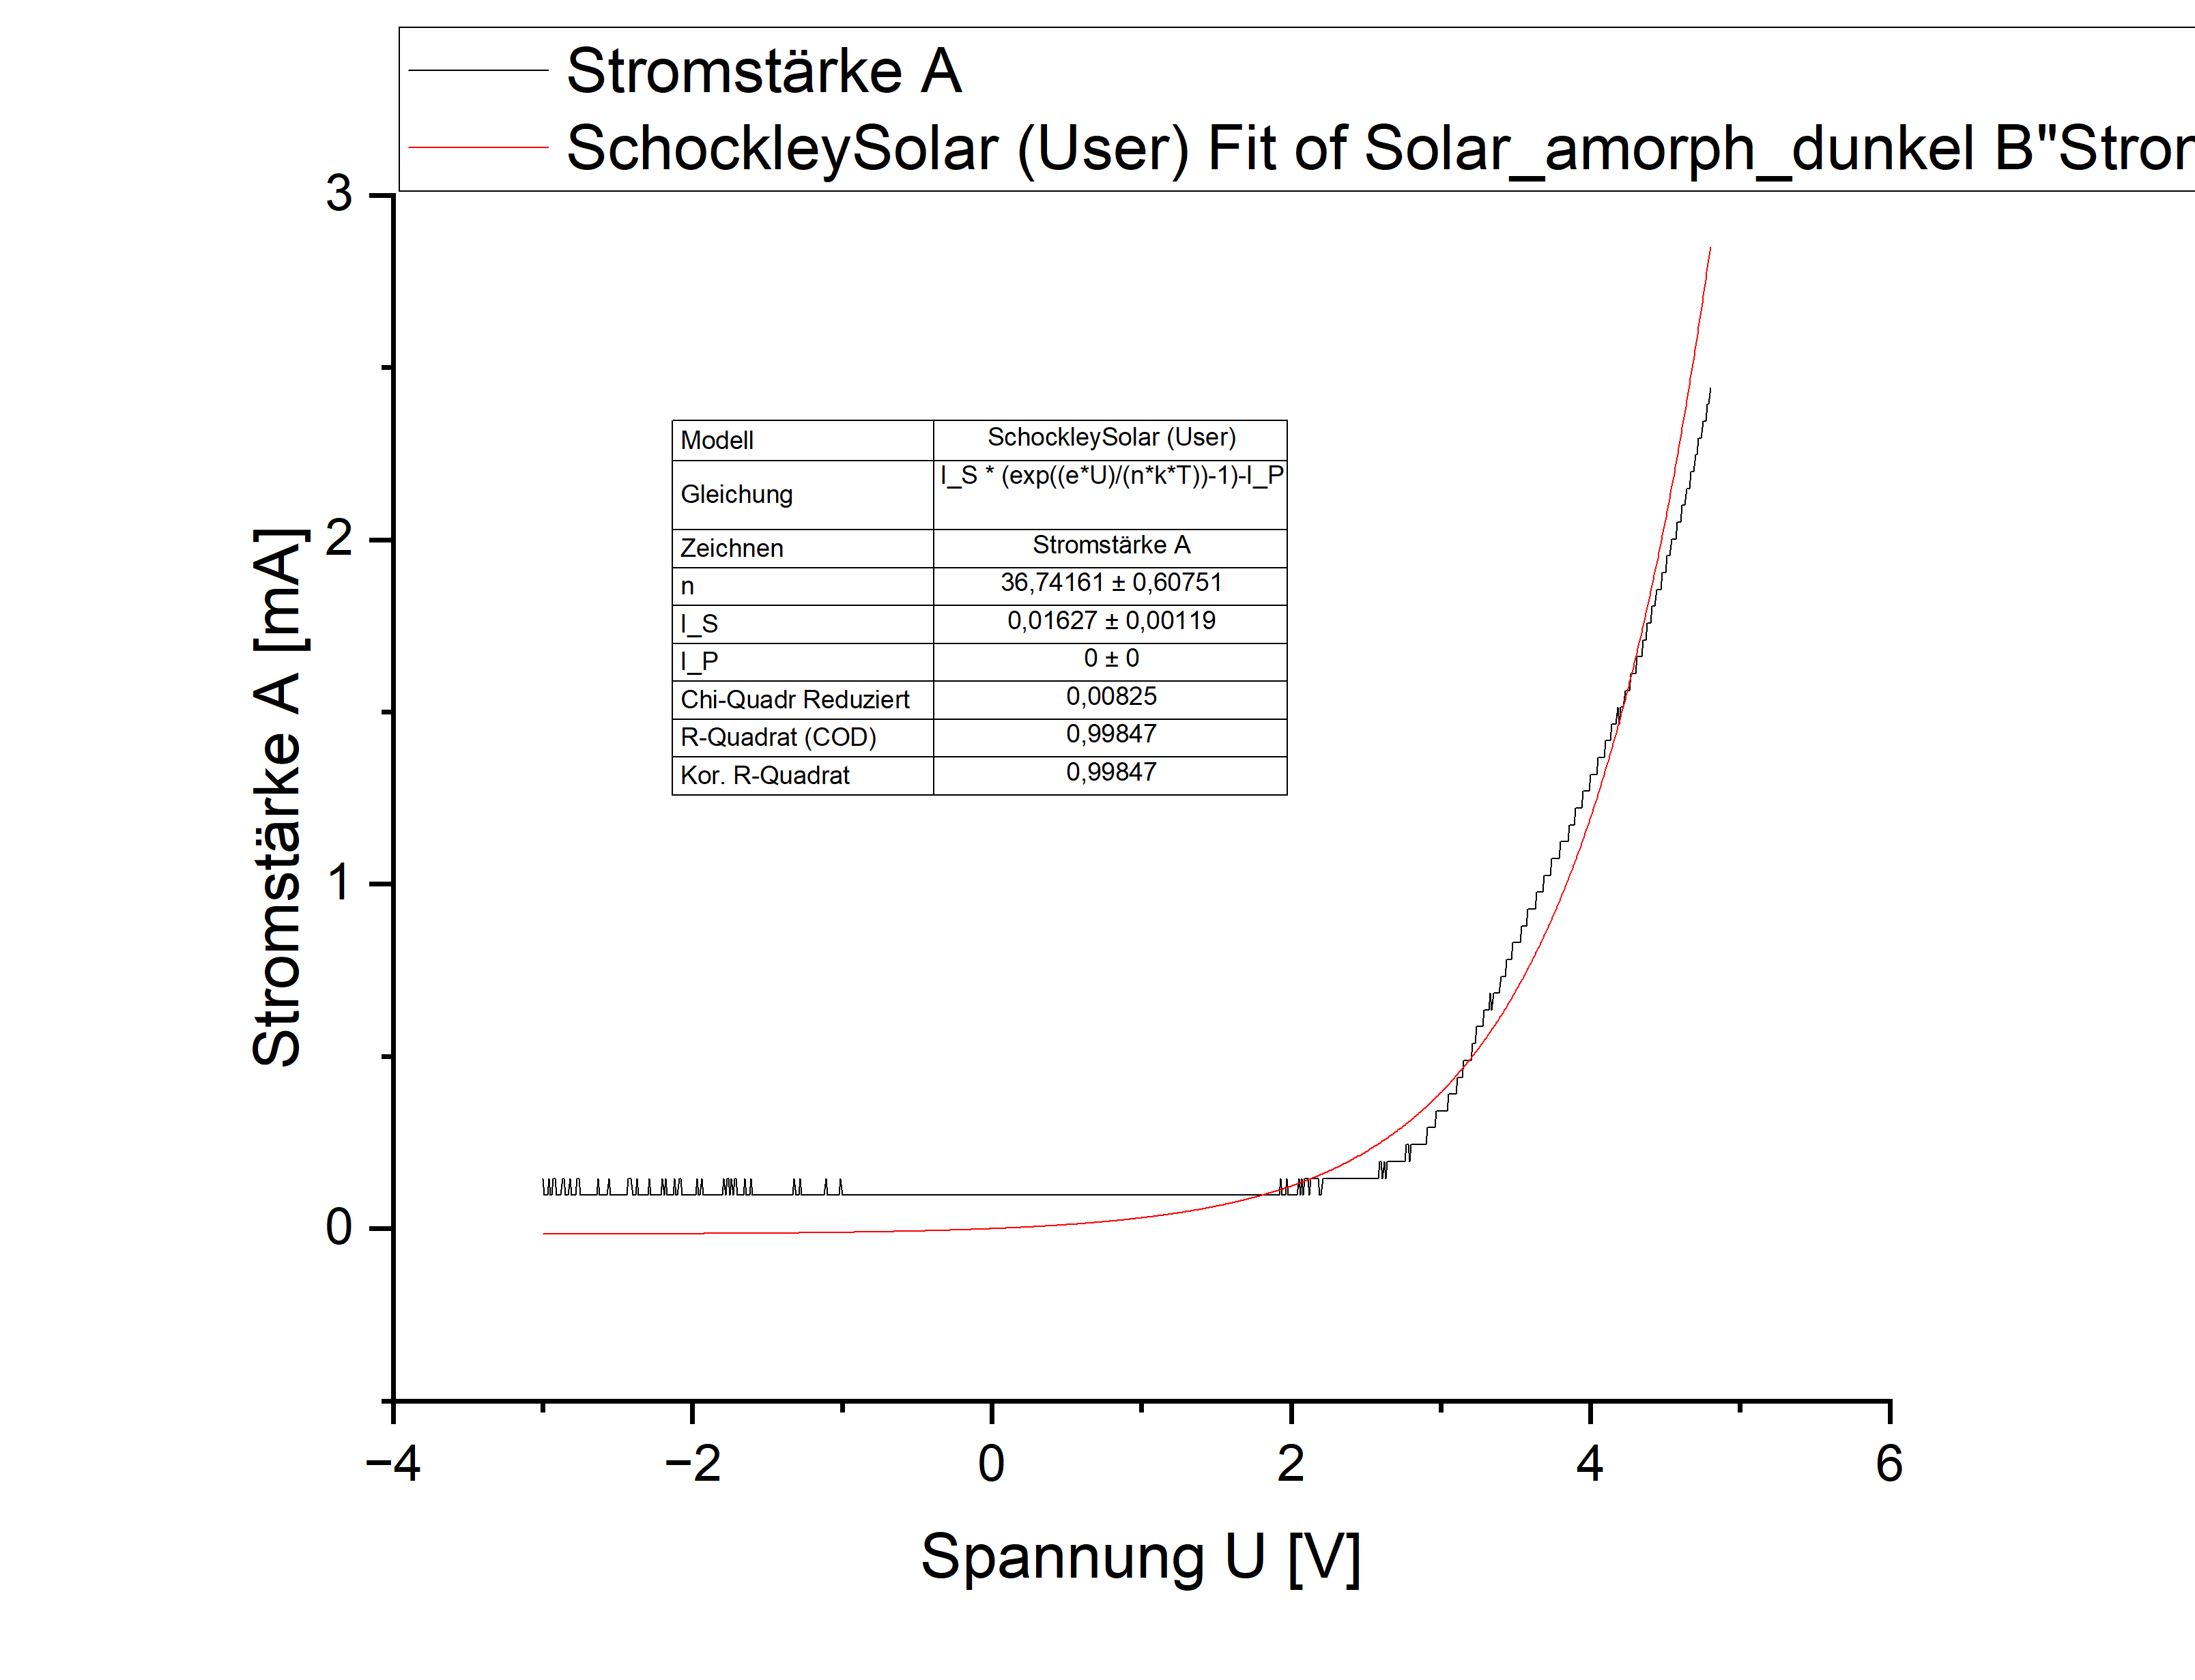
\includegraphics[width=0.8\textwidth]{Origin/Solar_amorph_dunkel.png}
			\caption{Kennlinie der amorphen Solarzelle im Dunkeln}
			\label{fig:SolarAmorphDunkel}
		\end{figure}

		\begin{figure}
			\centering
			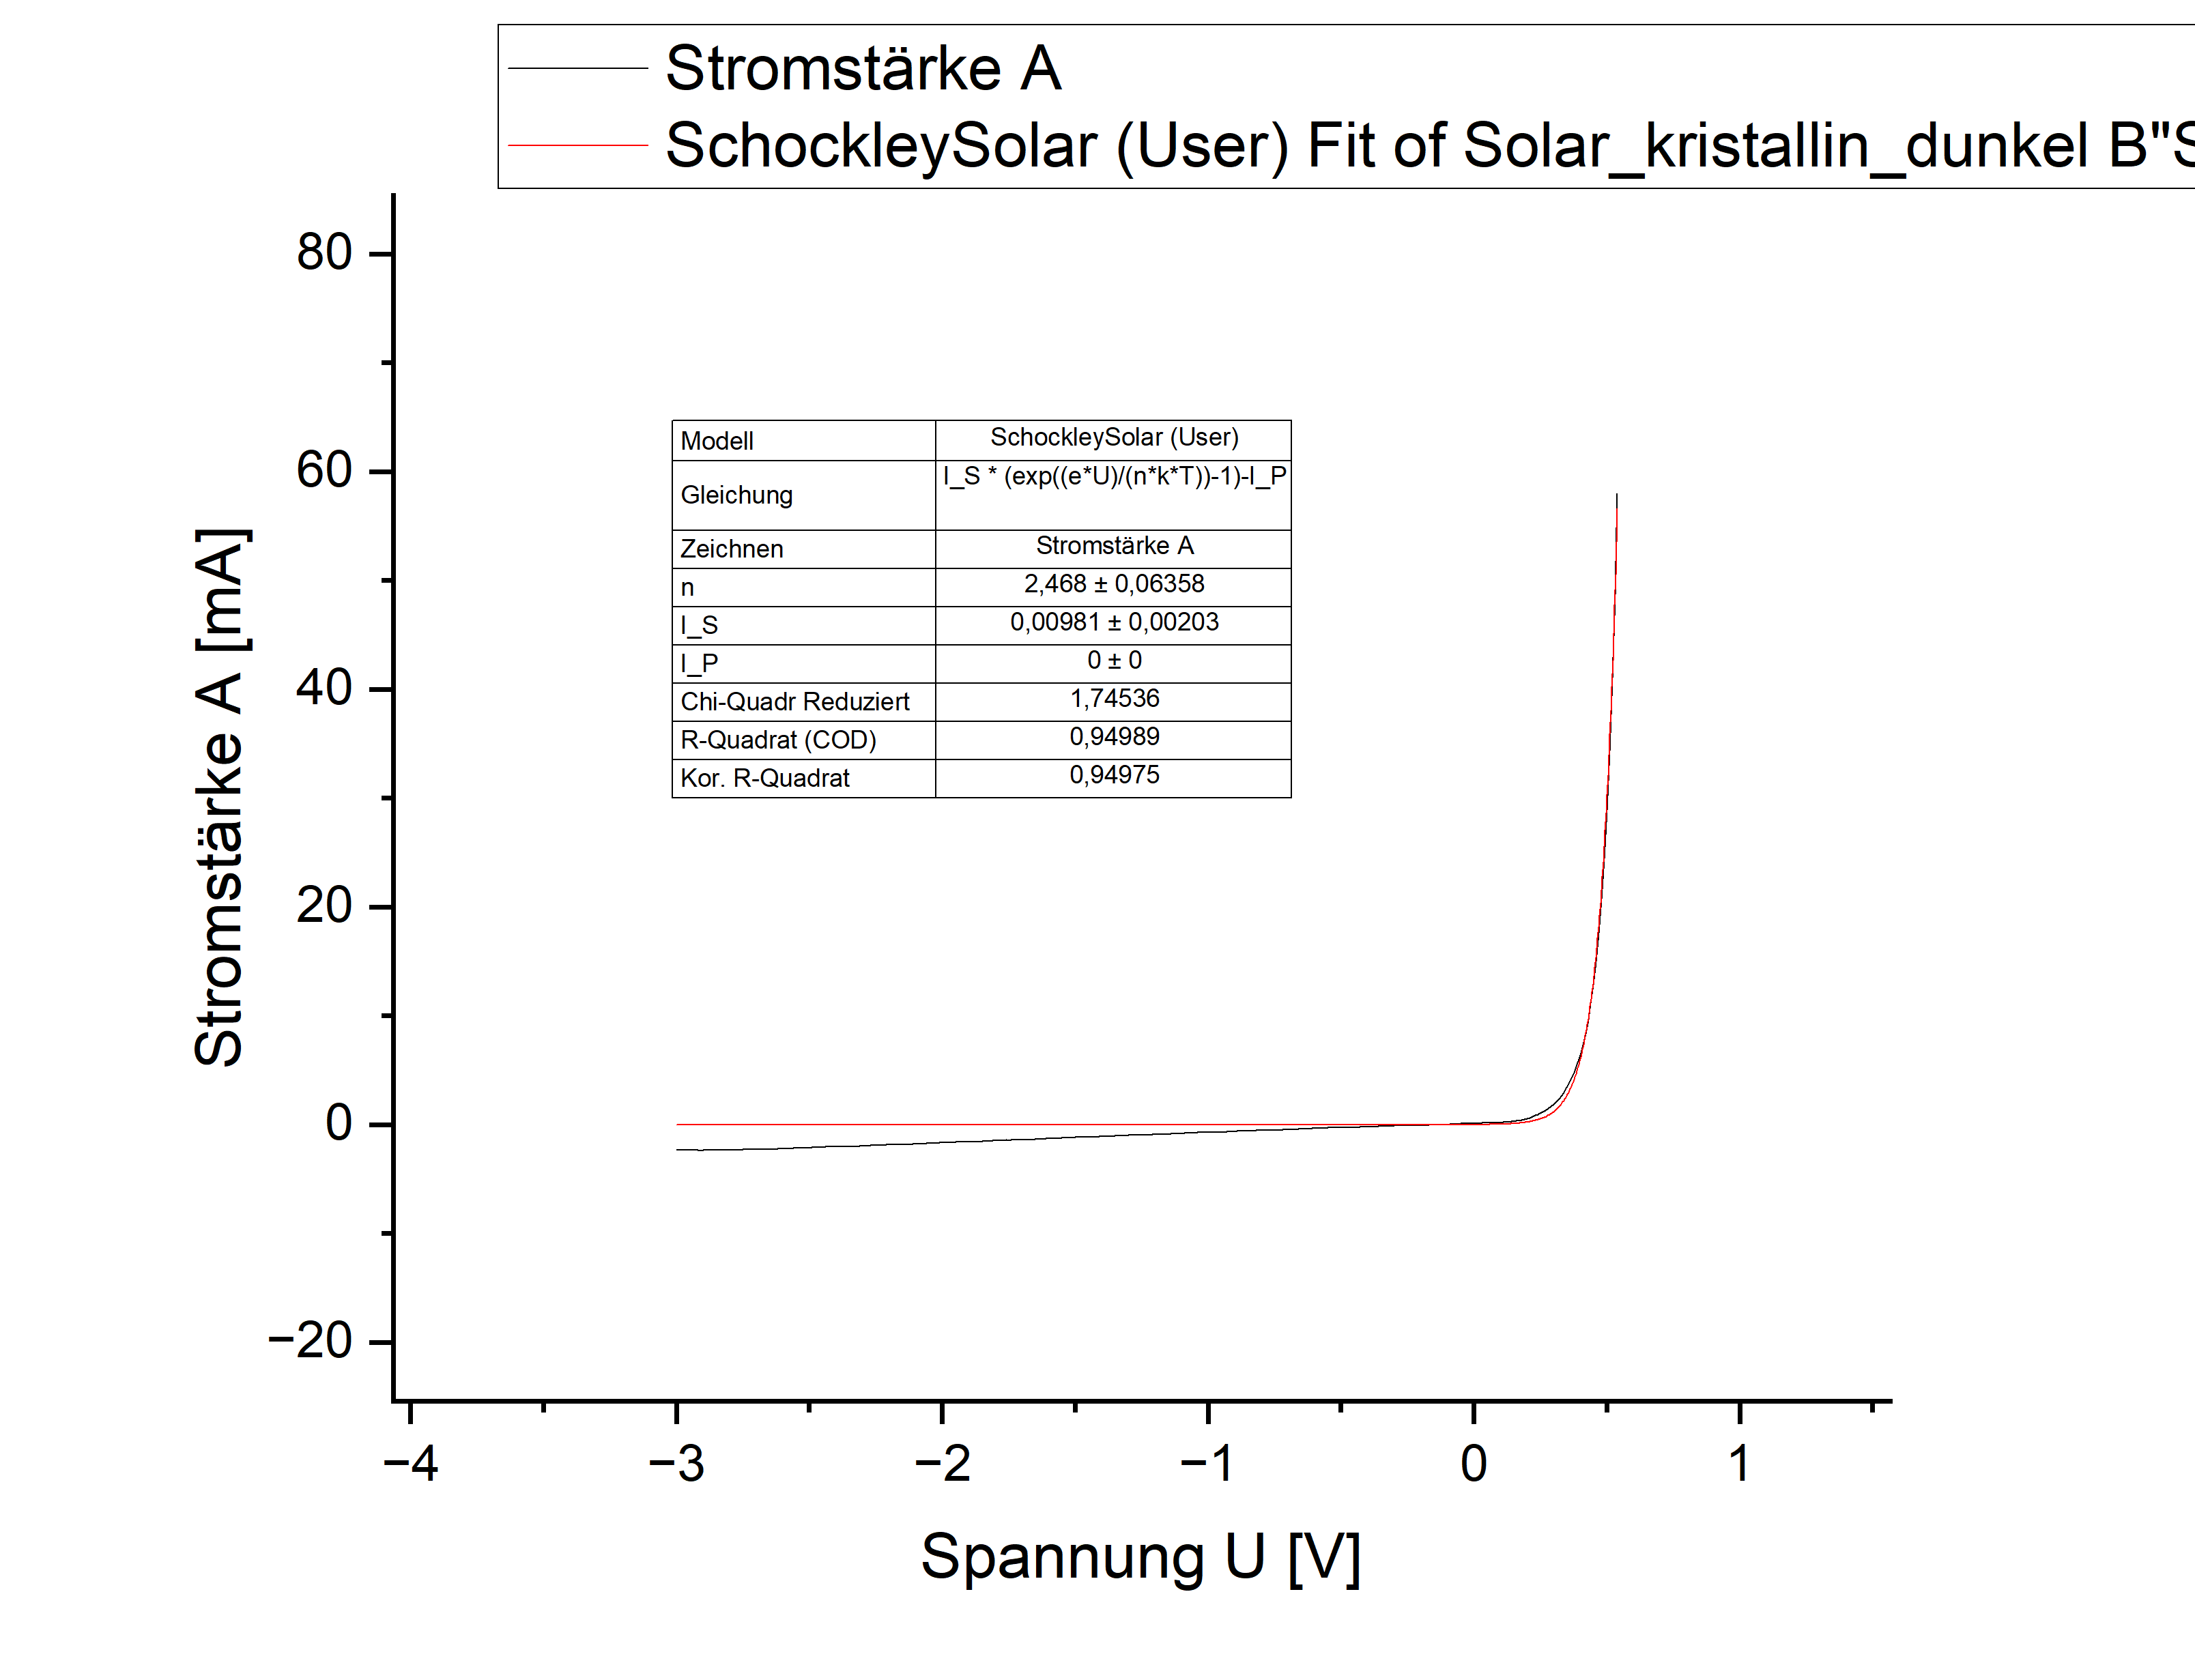
\includegraphics[width=0.8\textwidth]{Origin/Solar_kristallin_dunkel.png}
			\caption{Kennlinie der kristallinen Solarzelle im Dunkeln}
			\label{fig:SolarKristallinDunkel}
		\end{figure}


		\begin{samepage}
		\begin{itemize}
			\item Amorphe Solarzelle:
				\begin{itemize}
					\item Sättigungsstrom $I_\text{S} = \SI{0,01627+-0,00119}{\milli\ampere}$
					\item Emissionskoeffizient $n = \num{36,742 +- 0,608}$\\
					\item Die amorphe Solarzelle zeigt starke Abweichungen
zur idealen Diode auf. Dies ist auch zu erwarten, da in der Zelle keine Fernordnung
existiert, und sie somit einer idealen Diode recht unähnlich ist.
				\end{itemize}
			\item Kristalline Solarzelle:
				\begin{itemize}
					\item Sättigungsstrom $I_\text{S} = \SI{0,00981+-0,00203}{\milli\ampere}$
					\item Emissionskoeffizient $n = \num{2,468 +- 0,0636}$
					\item Die Ähnlichkeit zur idealen Diode lässt sich
auf den strukturellen Aufbau der Zelle zurückführen.
				\end{itemize}
		\end{itemize}
		\end{samepage}

	\subsection{Hellkennlinien}

		Aus dem Graph der Hellkennlinie, lassen sich die anderen Werte ablesen:
		
		\begin{description}
		\item[Der Kurzschlussstrom] I$_{SC}$ ist der Achsenabschnitt der vertikalen Achse, der nach Ablesen noch durch die Fläche der Zelle zu teilen ist. Im Fall der amorphen Zelle ist für diesen und andere Werte entweder ein Faktor (Strom) oder Divisor (Spannung) 5 hinzuzufügen, da es sich um fünf Einzelzellen handelt.
		\item[Die Leerlaufspannung] U$_{OC}$ ist der Achsnabschnitt der horizontalen Achse.
		\item[Der Füllfaktor] ergibt sich aus dem Minimum der Leistungs-Spannungs-Kurve. Der Punkt dieser Stelle im I-U-Diagramm ist der MPP. Der Füllfaktor ist dann $Ff=\frac{I_{MP}U_{MP}}{I_{SC}U_{OC}}$.
		\item[Der Wirkungsgrad] ist $\mu=\frac{\text{maximale Leistung}}{\text{Lichtleistung}}$.
		\end{description}
		
		
		\subsubsection{Kristalline Solarzelle}
		Die Solarzelle hat einen Durchmesser von \qty{5}{\centi\m} was eine Fläche von $\pi\cdot\num{2,5}^2=\qty{19,63}{\centi\m^2}$ entspricht. Die Werte der Solarzelle sind:
		
		\paragraph{Leerlaufspannung}
		\[	U_{OC} = \qty{0,472}{\volt} \]
		
		\paragraph{Kurzschlussstrom}
		$$\left|\frac{I_{SC}}{A}\right|=\frac{\qty{23,9}{\milli\ampere}}{\qty{19.63}{\centi\square\metre}}\approx\qty{1.22}{\milli\ampere\per\centi\square\metre} $$
		
		\paragraph{MPP} Siehe hierzu Graph \ref{fig:Leistkrishell}
		$$U_{MP}=\qty{0,36}{\volt}$$ $$\vert I_{MP}\vert=\qty{20,264}{\milli\ampere}$$ 
		Dieser Punkt impliziert eine Leistung von \qty{7,295}{\milli\watt}.

		\begin{figure}
			\centering
			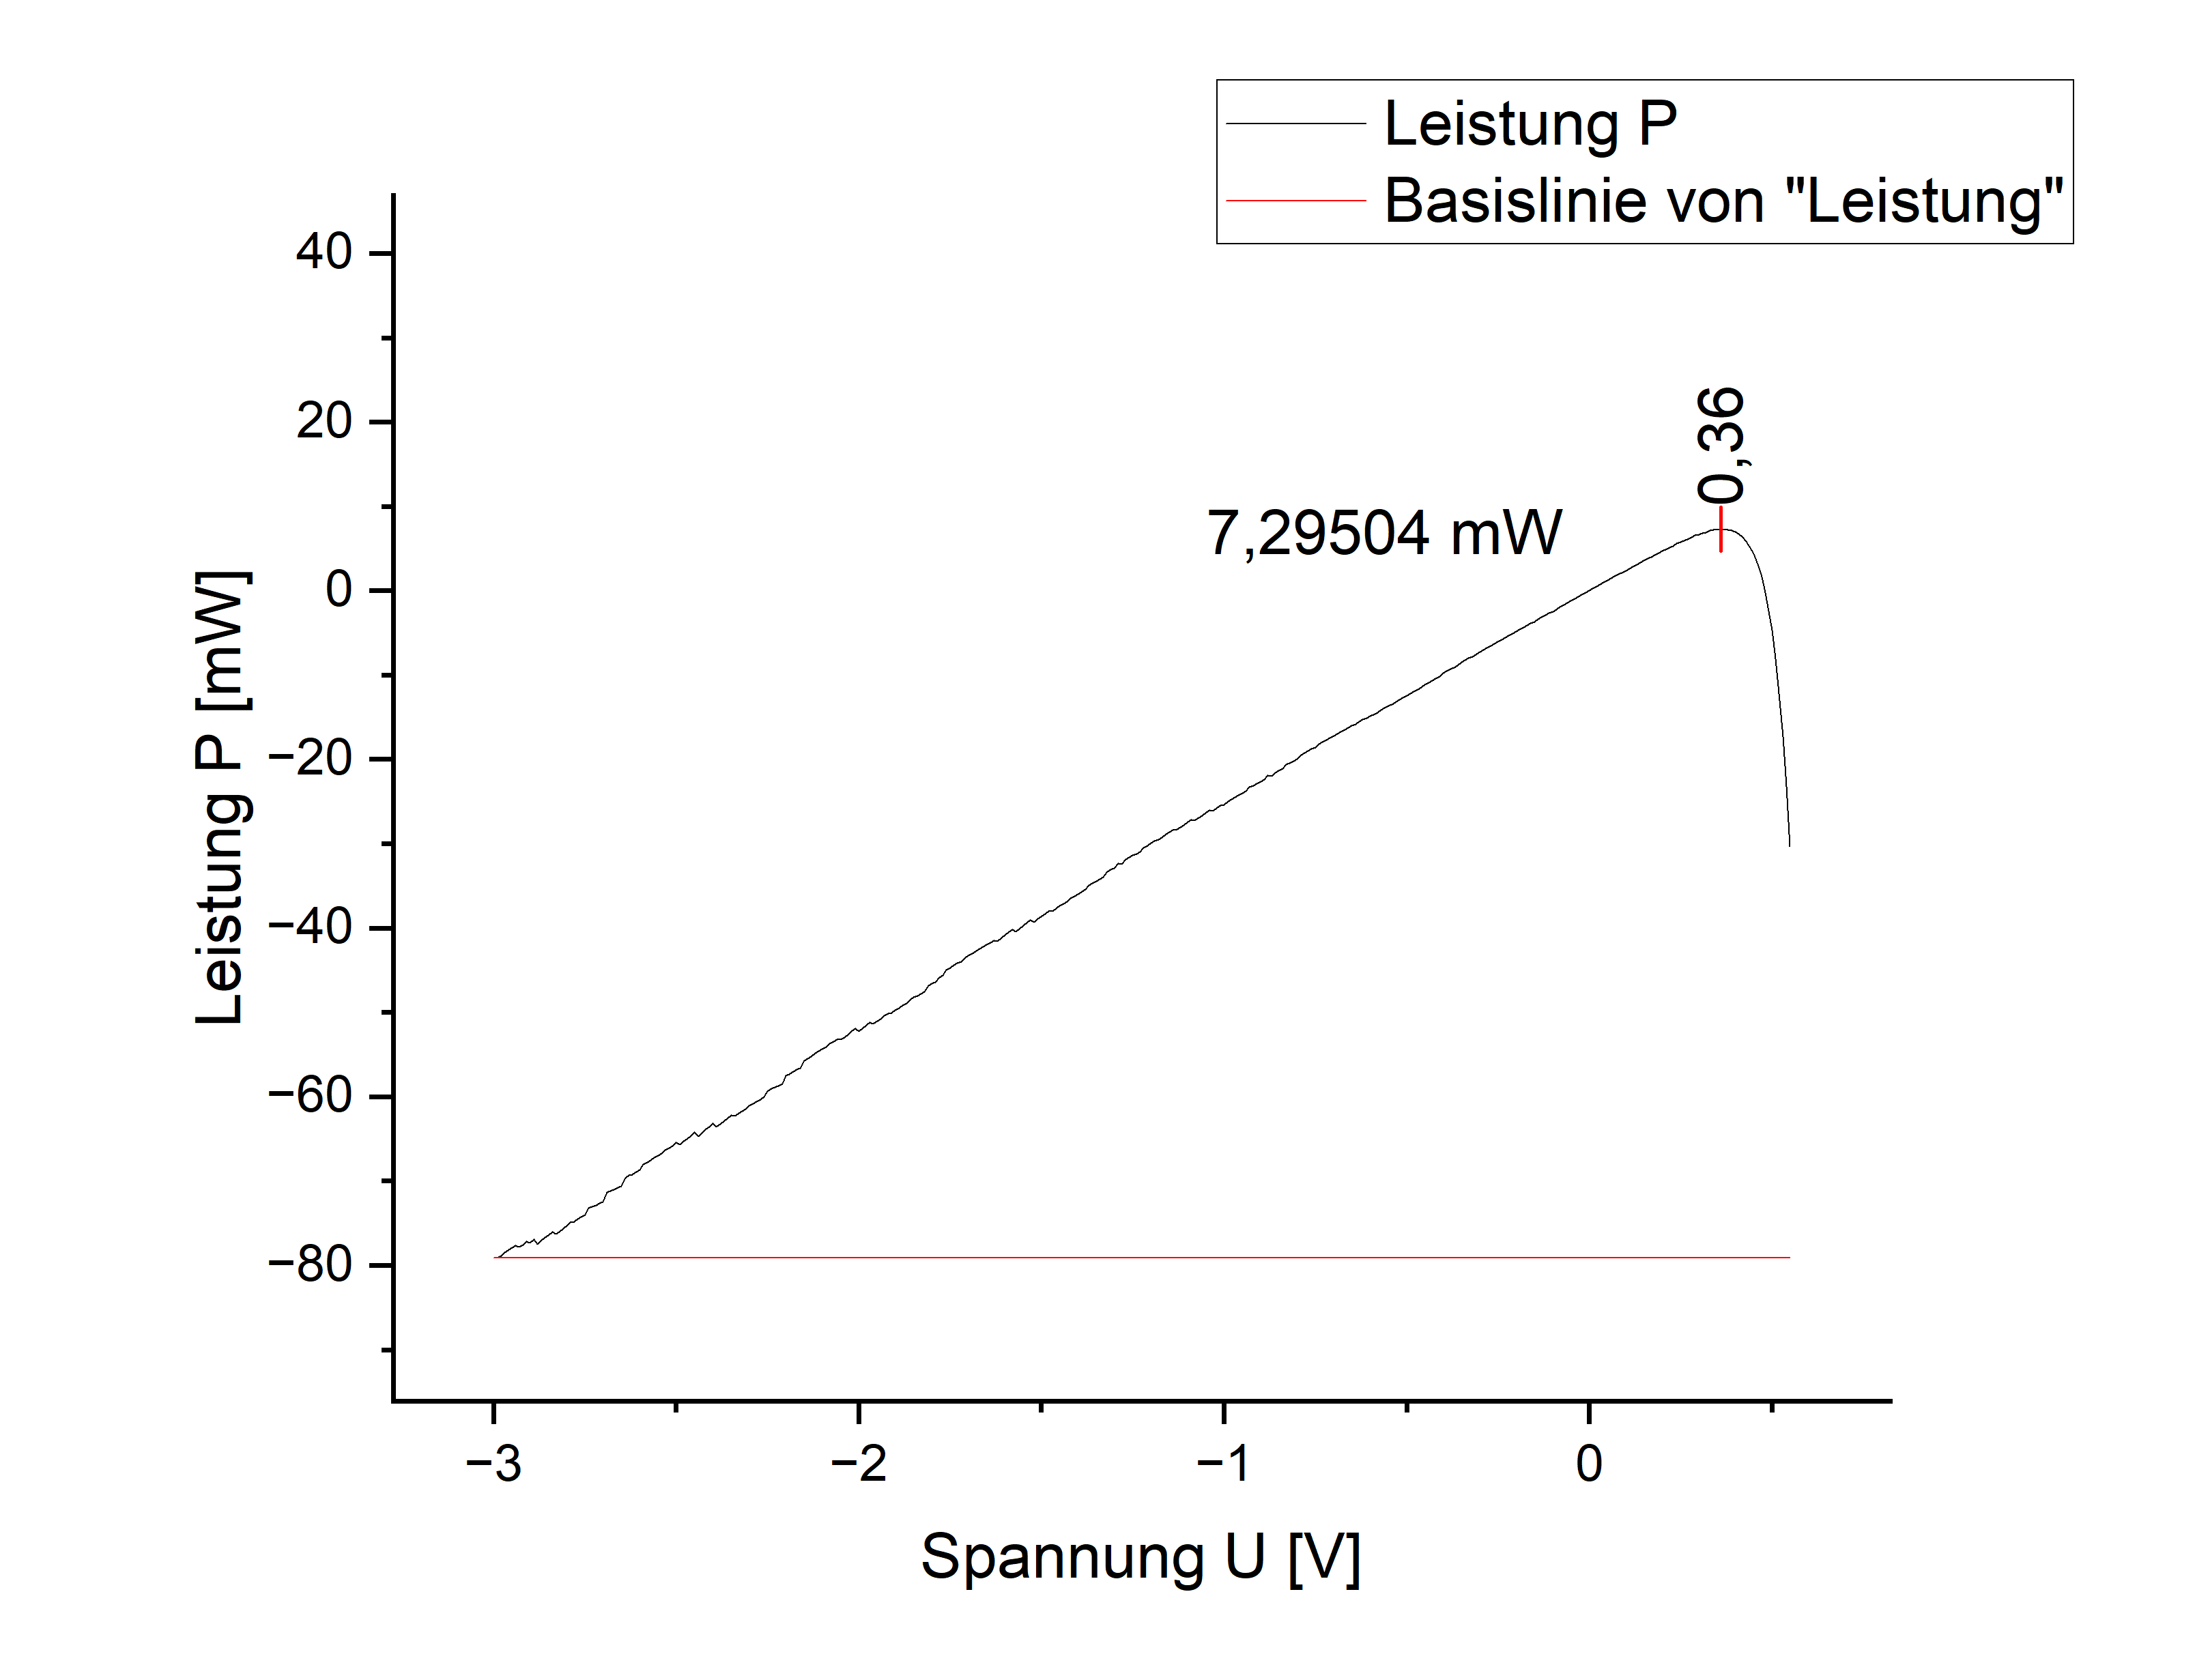
\includegraphics[width=0.8\textwidth]{Origin/LeistungKristall.png}
			\caption{Leistungskennlinie der kristallinen Solarzelle im Licht}
			\label{fig:Leistkrishell}
		\end{figure}
		
		\paragraph{Füllfaktor}
		
		$$    Ff=\frac{I_{MP}U_{MP}}{I_{SC}U_{OC}}= \frac{\qty{20,264}{\milli\ampere}\cdot \qty{0,36}{\volt}}{\qty{23,9}{\milli\ampere} \cdot \qty{0,472}{\volt}} = \num{0,646678} \approx \qty{64,67}{\percent}  $$
		
		\paragraph{Der Wirkungsgrad} ist über die Leistung der Lampe zu errechnen. Auf einen Messkopf mit einem Durchmesser von $\SI{1}{\centi\m} = \qty{0,01}{\m}$ strahlt die Lampe am Ort der Messung (der Solarzellen und des Messkopfs) eine Leistung von $P = \SI{9,2}{\milli\watt} $ ab. Das entspricht einer Leistungsdichte von $\frac{P}{A} = \frac{\qty{9,2}{\milli\watt}}{\pi\cdot(\qty{0,005}{\m})^2} = \frac{\qty{9,2}{\milli\watt}}{\qty{7,854e-5}{\square\metre}} = \qty{117,138}{\watt\per\m} $\\
		Auf Die Solarzelle fällt also eine Leistung von:
		\[P_ {belecht} = \qty{117,138}{\watt\per\m} \cdot \qty{19,63}{\centi\m^2} = \qty{22,99}{\watt}\]
		
		Der Wirkungsgrad ist somit:
		$$
		\eta=\frac{P_{MMP}}{P_{beleucht}} = \frac{\qty{7,295}{\milli\watt}}{\qty{22,99}{\watt}} = \num{3,173e-4} \approx \qty{0,03}{\percent}.
		$$
		Die Kennlinie der Solarzelle ist in Abbildung \ref{fig:SolarKristallinHell} zu sehen.\\
		
		\begin{figure}
			\centering
			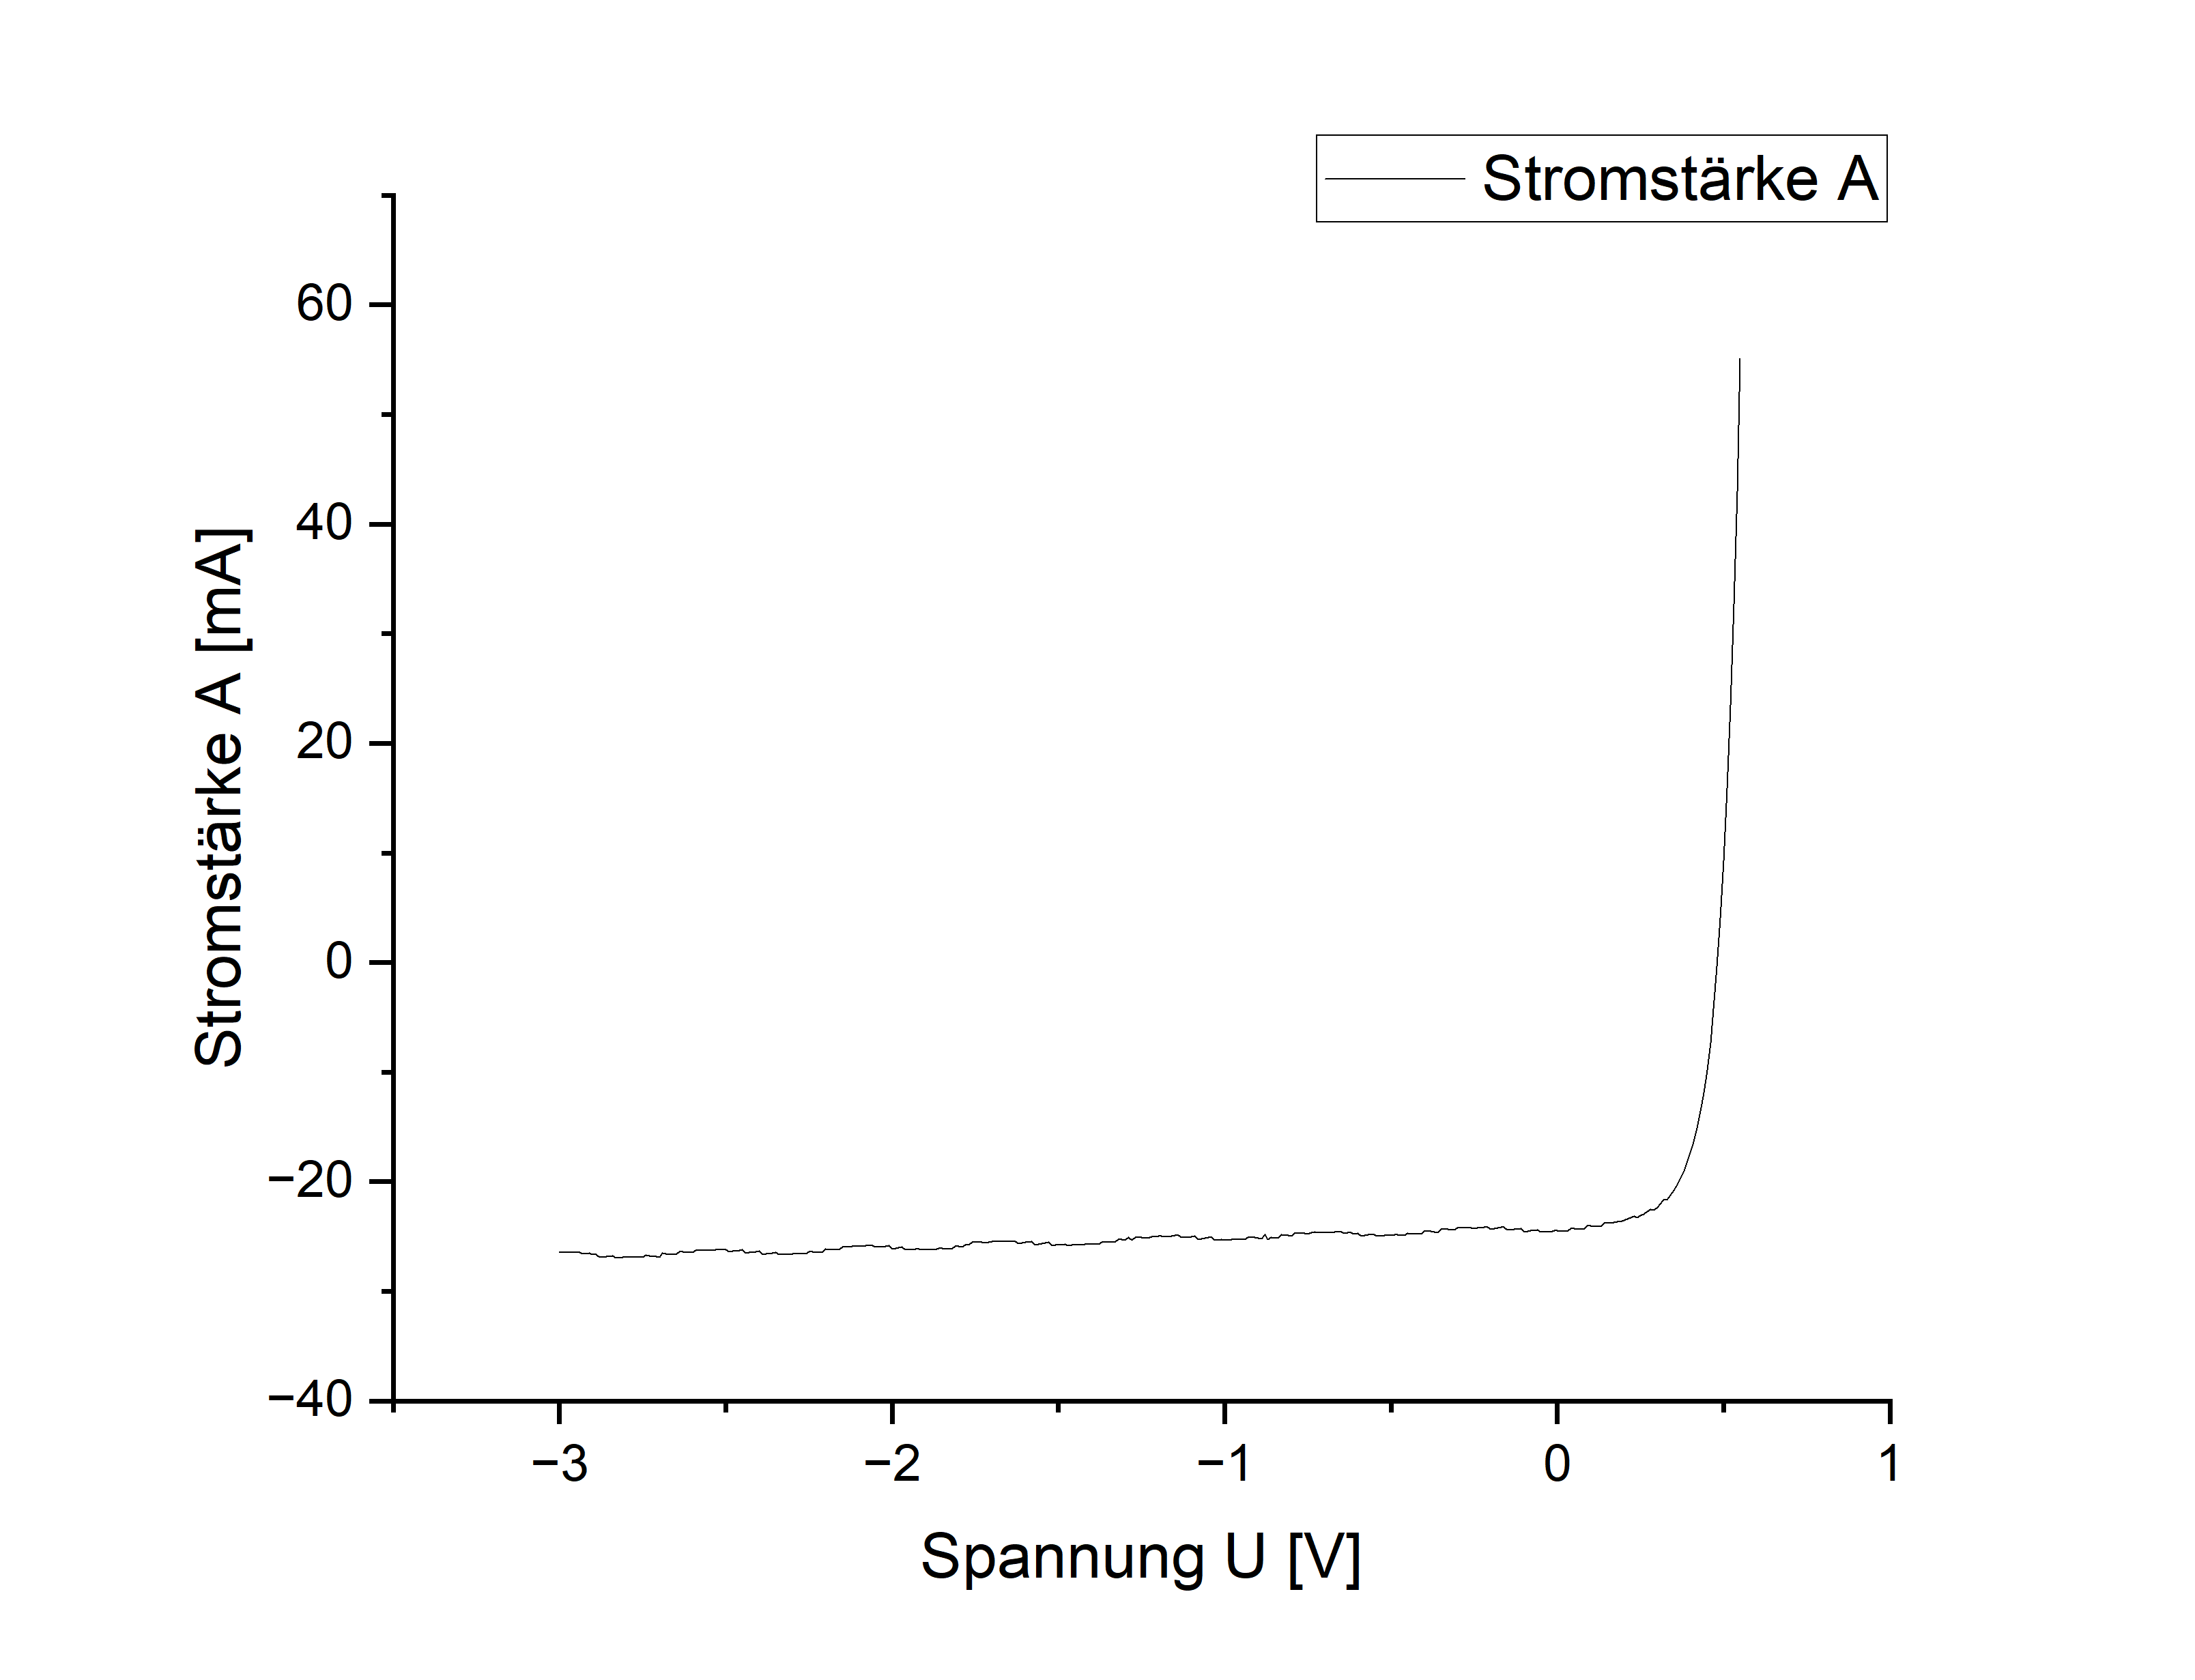
\includegraphics[width=0.8\textwidth]{Origin/SolarKristallHell.png}
			\caption{Kennlinie der kristallinen Solarzelle im Licht}
			\label{fig:SolarKristallinHell}
		\end{figure}
				
		
		\subsubsection{Amorphe Solarzelle}
		Die Solarzelle hat die Maße: \qty{2.2}{\centi\m} x \qty{2.8}{\centi\m} was einer Fläche von \qty{6,16}{\centi\square\metre} entspricht. Die Werte der Solarzelle sind:
		
		\paragraph{Leerlaufspannung}
		\[	U_{OC} = \frac{\qty{3,076}{\volt}}{5} = \qty{0,6352}{\volt} \]
		Man beachte, dass man hier durch die Anzahl der verwendeten Einzelzellen teilen muss,
		
		\paragraph{Kurzschlussstrom}
		$$\left|\frac{I_{SC}}{A}\right|=\frac{\qty{735}{\micro\ampere}}{\qty{6,16}{\centi\square\metre}}\cdot 5  \approx\qty{0,597}{\milli\ampere\per\centi\square\metre}$$
		
		\paragraph{MPP} Siehe hierzu Graph \ref{fig:Leistamorphhell}
		$$U_{MP}=\qty{2,35}{\volt}$$ $$\vert I_{MP}\vert=\qty{0,537}{\milli\ampere}$$ 
		Dieser Punkt impliziert eine Leistung von \qty{1,262}{\milli\watt}.
		
		\begin{figure}
			\centering
			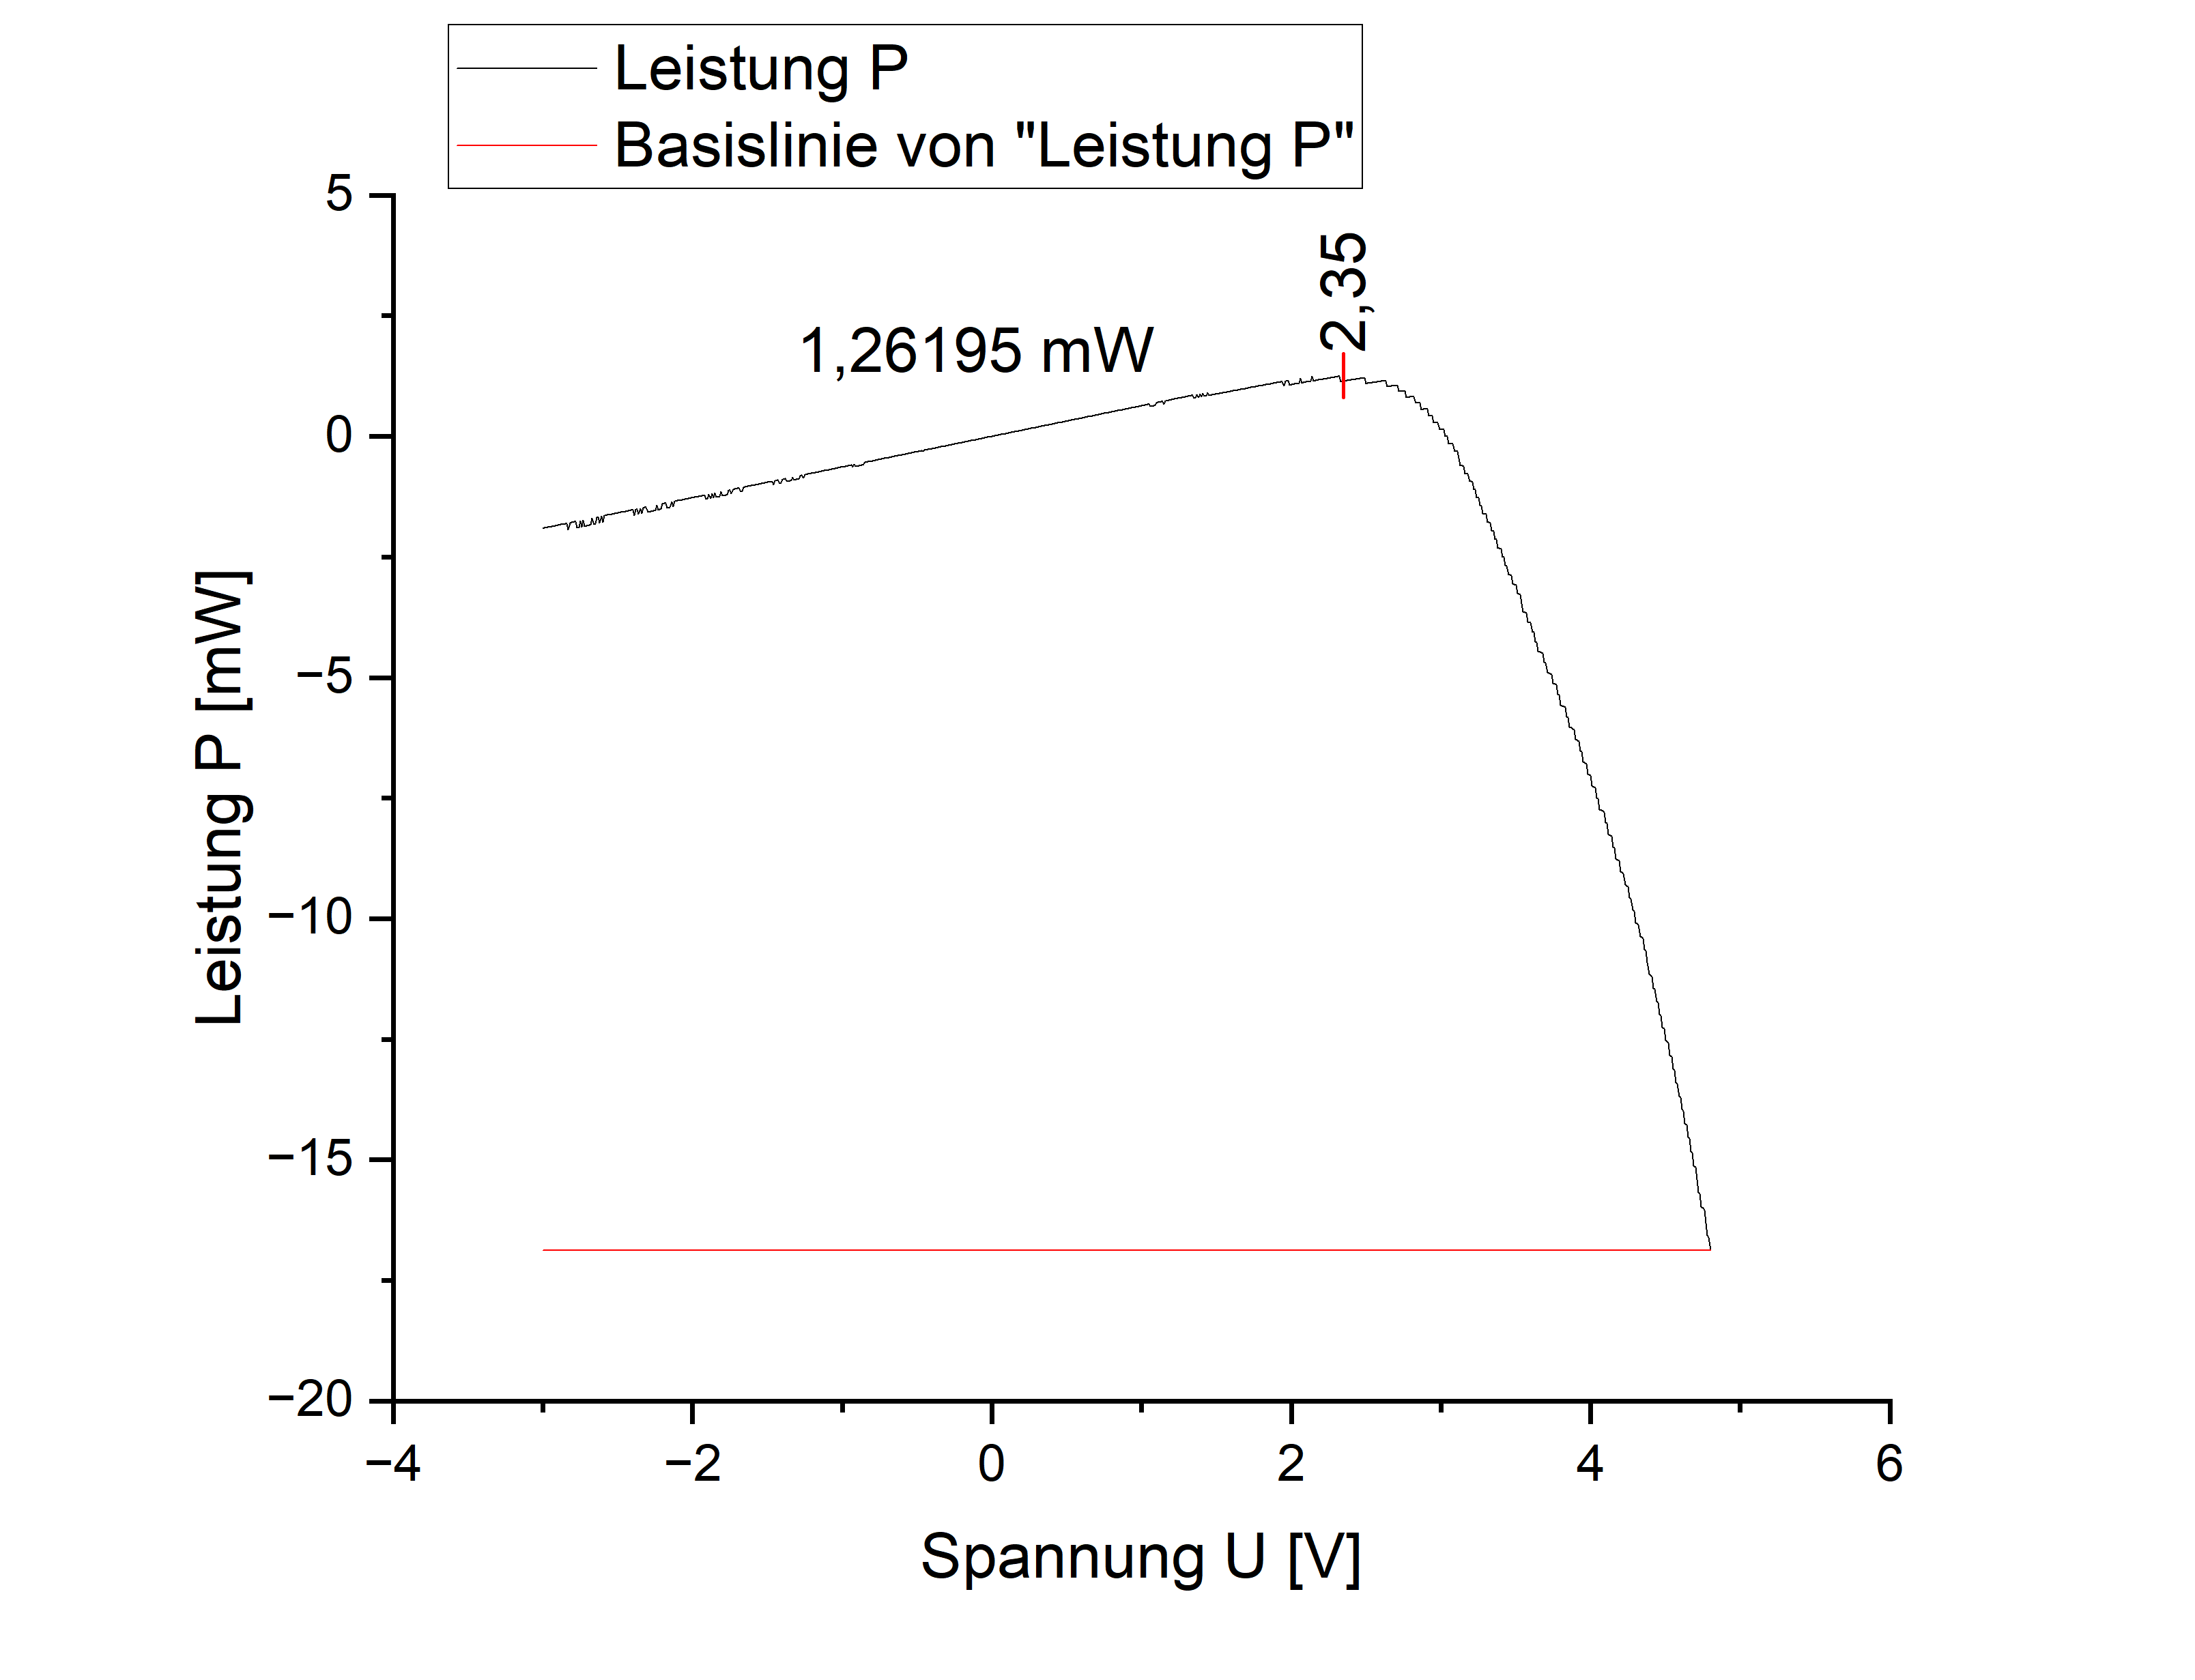
\includegraphics[width=0.8\textwidth]{Origin/LeistungAmorph.png}
			\caption{Leistungskennlinie der amorphen Solarzelle im Licht}
			\label{fig:Leistamorphhell}
		\end{figure}
		
		\paragraph{Füllfaktor}
		
		$$    Ff=\frac{I_{MP}U_{MP}}{I_{SC}U_{OC}}= \frac{\qty{0,537}{\milli\ampere}\cdot \qty{2,35}{\volt}}{\qty{3,675}{\milli\ampere} \cdot \qty{0,6352}{\volt}} = \num{0,5406} \approx \qty{54,06}{\percent}  $$
		
		\paragraph{Der Wirkungsgrad} ist über die Leistung von \qty{117,138}{\watt\per\m} der Lampe zu errechnen.\\
		Auf Die Solarzelle fällt dann eine Leistung von:
		\[P_ {belecht} = \qty{117,138}{\watt\per\m} \cdot \qty{6,16}{\centi\m\squared} \approx \qty{7,22}{\watt}\]
		
		Der Wirkungsgrad ist somit:
		$$
		\eta=\frac{P_{MMP}}{P_{beleucht}} = \frac{\qty{1,262}{\milli\watt}}{\qty{7,22}{\watt}} = \num{1,74792e-4} \approx \qty{0,017}{\percent}.
		$$
		Die Kennlinie der Solarzelle ist in Abbildung \ref{fig:SolarAmorphHell} zu sehen.\\
		
		\begin{figure}
			\centering
			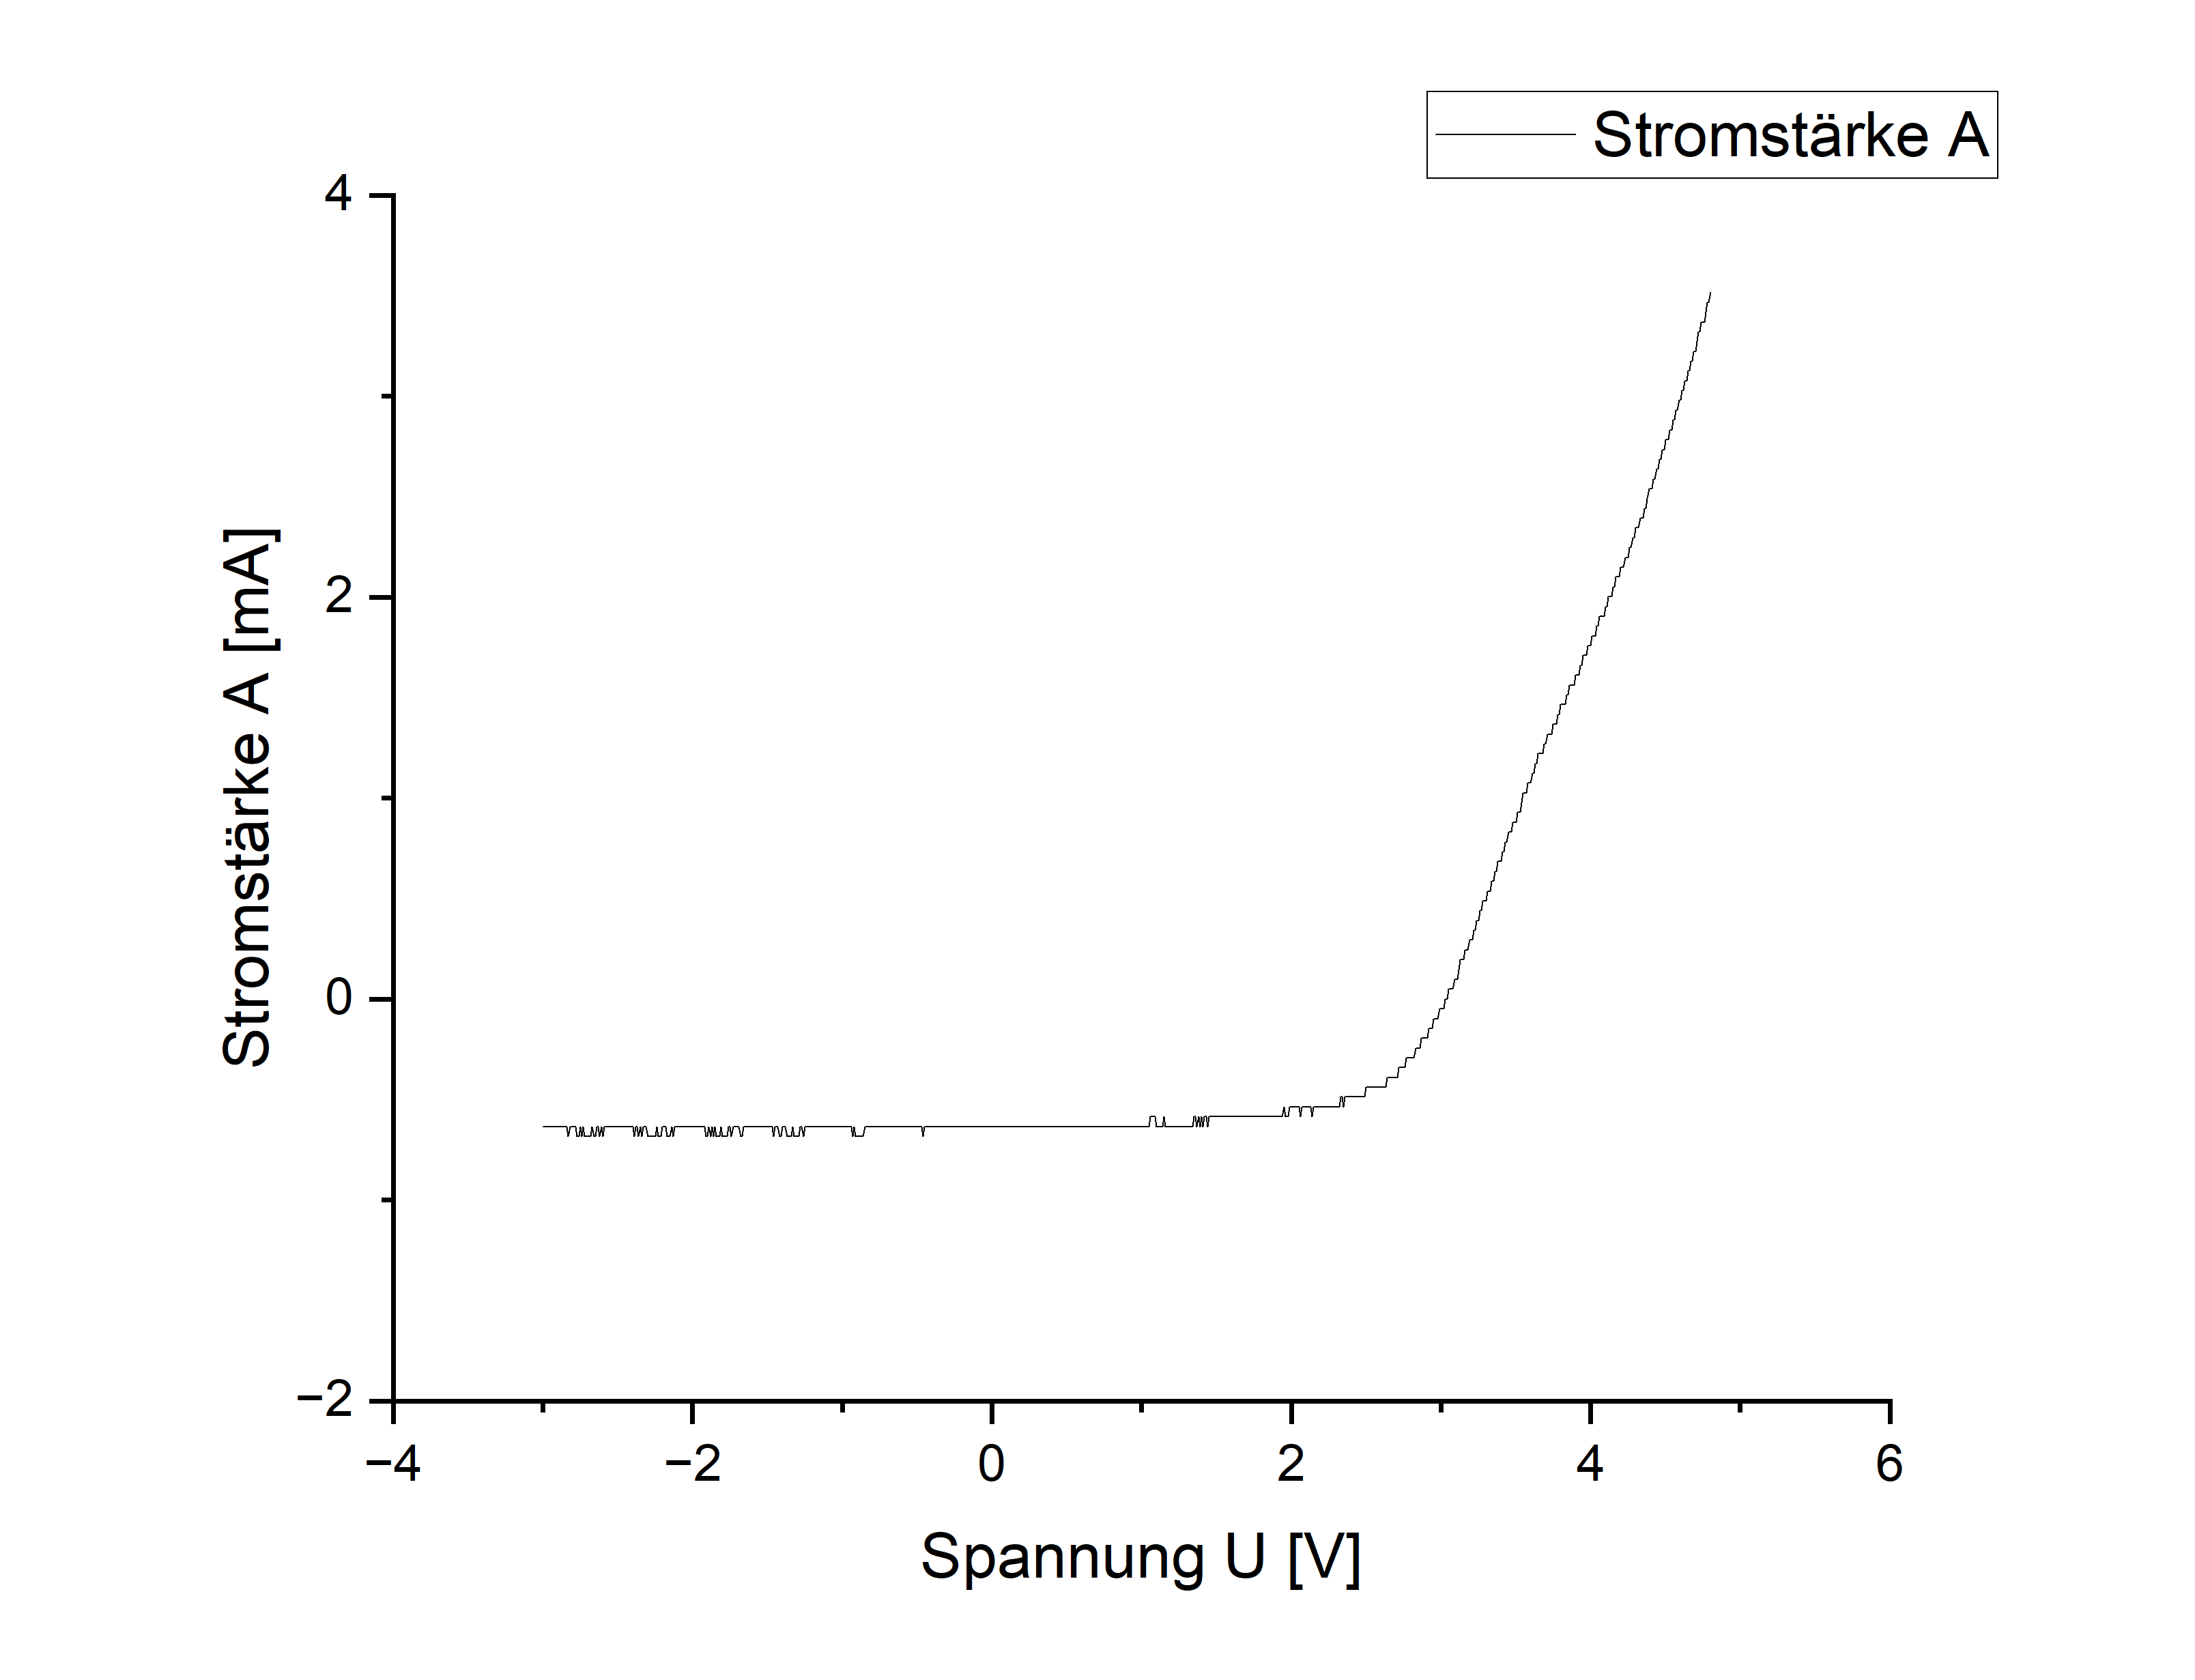
\includegraphics[width=0.8\textwidth]{Origin/SolarAmorphHell.png}
			\caption{Kennlinie der amorphen Solarzelle im Licht}
			\label{fig:SolarAmorphHell}
		\end{figure}
		
		

		


		
		



\chapter{Fazit}
In diesem Protokoll zu $U$-$I$-Kennlinien von Halbleiterbauelementen, konnten Einblicke in die Funktionsweise dieser gewonnen und charakteristische Eigenschaften der Bauelemente bestimmt werden.\\
Im Fall der Diode konnte ihr Verhalten als Gleichrichter beobachtetet werden, da die Kennlinie in Durchlass- und Sperrrichtung ein anderes Verhalten aufweist. Durch das Fitten der Shockley-Gleichung, wurden der Sättigungsstrom und Emissionskoeffizient bestimmt.\\
Für den Bipolartransistor wurde ein Vierquadrantenfeld aufgenommen und durch einen gewählten Arbeitspunkt die Vierpolparameter des Transistors bestimmt. Dafür wurde nicht direkt der jeweilige Anstieg am Arbeitspunkt verwendet, sondern ein Bereich um diesen, da es sich um Messdaten handelt und diese natürlicherweise Schwankungen aufweisen. Mit einem Stromverstärkungsfaktor von rund 200, wurde ein sehr typischer Wert für Kleinsignaltransistoren in der Emitterschaltung bestimmt werden. An diesem Wert wird deutlich, das Transistoren nicht nur als elektrische Schalter genutzt werden können, sondern auch als Verstärker, so finden sie zum Beispiel Anwendung in den Schaltungen von Operationsverstärkern.\\
Der Feldeffekttransistor konnte klar als  Metall-Oxid-Feldeffekttransistors identifiziert werden, da er bei nicht angelegter Steuerspannung sperrend war und kein Strom geflossen ist. Der Vorteil von Feldeffekttransistoren gegenüber Bipolartransistoren ist, das sie quasi leistungslos gesteuert werden können, da sie spannungsgesteuert sind und kein Strom fließen muss.\\
Die Solarzellen hatten erstaunlich geringe Wirkungsgrade (wobei auch die anfängliche Beleuchtungsmessung fehlerhaft sein könnte) und nach unserer Messung hatte die kristalline Solarzelle einen höheren Wirkungsgrad.



	\listoffigures
	\addcontentsline{toc}{chapter}{\listfigurename}
	
	\begin{thebibliography}{111} \addcontentsline{toc}{chapter}{Literaturverzeichnis}
		\bibitem{Anleitung}
		I. Physikalisches Institut, \glqq Versuch 1.8: I-U-Kennlinien an Halbleitern
		und Solarzellen \grqq{}, 2024.
		
		\bibitem{beuth}
		K. Beuth, \glqq Elektronik 2 – Bauelemente\grqq, Vogel Buchverlag (Bauelemente)
		
		\bibitem{hunklinger}
		S. Hunklinger, \glqq Festkörperphysik\grqq, Oldenbourg Wissenschaftsverlag (Grundlagen)
		
		
		
	\end{thebibliography}


\chapter*{Anhang} \label{ch:Anhang}
\addcontentsline{toc}{chapter}{Anhang}
\FloatBarrier





\end{document}
